\RequirePackage{fix-cm}
\documentclass[smallextended]{svjour3}
%
\smartqed
%
\usepackage{graphicx}
\graphicspath{{images/}}
\usepackage{etoolbox}
\usepackage{bm}
\usepackage{xcolor}
\usepackage{amsmath}
\usepackage{subfig}
\usepackage{multirow}
\usepackage{todonotes}
\usepackage{float}
\usepackage{hyperref}
\usepackage[numbers]{natbib}
\bibliographystyle{spphys}

% Placeholder box for figures whose final artwork is not yet inserted.
% Renders a framed grey panel with a short description, so the document
% compiles without the missing-file error and the layout is preview-able.
\newcommand{\figplaceholder}[2][0.30\textheight]{%
  \fboxsep=0pt\relax
  \fbox{\parbox[c][#1][c]{0.92\linewidth}{\centering
      \color{gray}\itshape [\,Placeholder figure - #2\,]}}%
}

\begin{document}

\title{Topology-Locked Flow Organization in a Rotationally-Stacked Packed Bed: Pore-Scale Lattice-Boltzmann Simulation Validated by PIV}

\author{T. Neeraj         \and
        C. Velten         \and
        F. Gharibi        \and
        K. Z\"ahringer     \and
        D. Th\'evenin
}
\institute{T. Neeraj \at
              Tel.: +49-15214529344\\
              \email{tanya.neeraj@ovgu.de}
           \and
           C. Velten \at
           christin.velten@ovgu.de
}
\date{Received: date / Accepted: date}
\maketitle

\begin{abstract}
% TODO: write abstract last.
% Hook: first pore-scale LBM of Ref Config IIa validated against PIV across three
% topologies; introducing a quantitative order parameter for layer-periodic flow
% locking; irregular case as a clean control.
\keywords{Lattice Boltzmann \and Packed bed \and porous media \and flow locking \and PIV validation}
\end{abstract}

%% ============================================================
\section{Introduction}
\label{sec:intro}

% Transport in structured/rotational porous media; importance of pore-scale flow
% organisation for mixing, transport, reactor performance.
% Limits of Darcy/volume-averaged models.
% Deterministic rotational topology as a design knob.
% Prior work: PIV \cite{velten2026}; FVM (Sadowski et al.) noted qualitative
% layer-repeatability and antisymmetry  never quantified.
% Gap = a quantitative, validated, multi-topology description of locking.
% Objectives and contributions.
\todo[inline]{Write Introduction}

%% ============================================================
\section{Experimental Setup}
The experimental reference configuration is described in detail by~\citet{velten2026}. The packing consists of polyhedral bar modules, each containing five parallel bars of height $l_\mathrm{ch} = 10\,\mathrm{mm}$ separated by slits of width $l_P = 5\,\mathrm{mm}$, housed within a circular cross-section of diameter $d_\mathrm{inlet} = 62.12\,\mathrm{mm}$ (Fig.~\ref{fig:geometry}. The volume fraction of the void (porosity), defined as the volume of the void relative to the volume of the overall module, is $\varphi = 0.332$. Modules are 3D-printed from PA \,12 by laser sintering (tolerance $0.3\%$) and can rotate against each other in increments of $5^\circ$ by $37$ indexing slits on the rim, spanning $0$-$180^\circ$~\citep{velten2026}.
The parallel-bar geometry is what enables direct optical access: in the experiment three of the five  bars in the measurement module are replaced by transparent fused-silica glass bars, so that a laser light sheet can be introduced through the void spaces and the camera can view the interior pores without refractive-index matching~\citep{velten2026}. 

In the experiment the bed is bounded by a gas inlet zone - a diffuser filled with $3\,\mathrm{mm}$ glass beads followed by a tranquilisation zone that distributes the flow homogeneously over the circular cross-section $A = 3031\,\mathrm{mm^2}$ - and, on top of the $18$th layer, a rectangular optical outlet box ($70\times70\,\mathrm{mm^2}$
windows, height $200\,\mathrm{mm}$) that minimises the influence of the surroundings on the bed-surface flow~\citep{velten2026}. The present simulations do not resolve this inlet with so many extra diffusor parts. Instead, the diffuser and tranquilisation zone are replaced by a uniform inlet of the same circular cross-section as the bed, extended upstream by a short straight section ($60\,\mathrm{mm}$) sufficient for the velocity profile to homogenise before it reaches the first module. This reproduces the experimentally intended uniform feed while avoiding the grid cost of meshing the bead-packed diffuser, substantially reducing the geometric complexity and node count of the computational domain.

\begin{figure}[h]
\centering
\figplaceholder{apparatus and packing: optical-access reactor with five parallel
bars per module, the spiral inner pore network of the $30^\circ$ stack, and the
transparent glass bars enabling laser light-sheet access (after Fig.~2 of
\citealt{velten2026})}
\caption{Geometry of the rotationally-stacked packed bed. Each module contains five
parallel bars (height $l_\mathrm{ch} = 10\,\mathrm{mm}$, slit width
$l_P = 5\,\mathrm{mm}$) housed in a circular cross-section of diameter
$d_\mathrm{inlet} = 62.12\,\mathrm{mm}$; successive modules are twisted by a fixed
angle $\theta$, producing the spiral inner pore structure. Adapted
from~\citet{velten2026} (CC~BY~4.0).}
\label{fig:geometry}
\end{figure}

\subsection{Twist-and-Repeat Topology}
\label{sec:geometry:topology}

Because the modules are identical and only their angular offset changes, the bed is generated by a single \emph{twist-and-repeat} rule: each module is the one below it, rotated about the column axis by a fixed angle $\theta$ and shifted up by one layer height $l_\mathrm{ch}$. The structure therefore possesses two competing geometric length scales. The first is the per-layer misalignment $\theta$, which controls how far an open slit (and hence a through-flowing jet) stays aligned before it is occluded by the bars of the next module. The second is a superlattice period: since the bar pattern of a single module is invariant under a $180^\circ$ rotation, the stack returns to its original orientation after
\begin{equation}
    N = \frac{180^\circ}{\theta}
    \label{eq:period}
\end{equation}
layers. For the regular $30^\circ$ configuration $\theta = 30^\circ$ gives $N = 6$, so six successive modules span $6\times30^\circ = 180^\circ$ and the seventh module repeats the orientation of the first~\citep{velten2026}. The $40^\circ$ configuration gives the longer period $N = 9$. The full bed of $18$ stacked modules (bed height $18\,l_\mathrm{ch} = 180\,\mathrm{mm}$) thus contains exactly three complete geometric periods of the $30^\circ$ packing, producing the spiral inner pore structure illustrated in Fig.~\ref{fig:geometry}. All optical measurements~\citep{velten2026}, and the simulation planes used for validation here, are taken in layers L13-L17, i.e.\ within the third (fully developed) period counted from the gas inlet at the bottom of the bed.

A consequence of the $180^\circ$ symmetry of the bar pattern is that the inner pore
network is point-symmetric between two layers: when two modules are rotated against each other, the first and fourth voids carry the same number of inlets as the second and third, and depending on $\theta$ between one and four through-passages connect a lower module to the one above it~\citep{velten2026}. The $30^\circ$ configuration realises a $2/3$ inlet pattern.

\subsection{Three Topologies Studied}
\label{sec:geometry:topologies}

The modularity of the reactor allows a continuum of pore structures to be assembled
from the same hardware simply by choosing the inter-layer rotation angle~\citep{velten2026}. We study three representative topologies here:
\begin{itemize}
    \item \textbf{$30^\circ$ (regular, period $N = 6$):} the experimentally measured benchmark configuration, with the shortest period and the longest jet-alignment length of the cases considered.
    \item \textbf{$40^\circ$ (regular, period $N = 9$):} a second periodic packing whose larger per-layer twist shortens the alignment length and lengthens the geometric period.
    \item \textbf{Irregular (aperiodic control):} successive layers are rotated by a non-repeating sequence of angles, so there is no twist-and-repeat rule and no
    superlattice period. This packing serves as a clean control: it shares the same bars, slits, porosity and bounding apparatus as the regular cases but lacks the geometric periodicity, and therefore cannot exhibit flow locking (Sec.~\ref{sec:locking}).
\end{itemize}

The particle Reynolds number is defined following~\citet{velten2026} as \begin{equation}
    Re_P = \frac{v_s\,\rho\,l_\mathrm{ch}}{\varphi\,\mu},
    \label{eq:rep}
\end{equation}
where $v_s$ is the superficial velocity, $\rho = 1.204\,\mathrm{kg/m^3}$ and $\mu = 1.822\times10^{-5}\,\mathrm{kg/(m\,s)}$ are the density and dynamic viscosity of air at $T = 20\,^\circ\mathrm{C}$ and $p = 1\,\mathrm{atm}$, and $l_\mathrm{ch} = 10\,\mathrm{mm}$ is the bar width~\citep{velten2026}. The superficial velocity follows from the volume flow rate $Q$ through $Q = A\,v_s$, with $A = 3031\,\mathrm{mm^2}$ the reactor cross-section.
In our study we have simulated $Re_P 100, 300, 500$. In the reference experiment $Re_P = 100$ correspond to $Q = 9.14$$\mathrm{L/min}$, $Re_P = 300$ correspond to $Q = 13.71$$\mathrm{L/min}$ and $Re_P = 500$ correspond to $Q = 45.72$$\mathrm{L/min}$~\citep{velten2026}.

The laminar $Re_P = 100$ case is run for all three topologies and provides the validation baseline; the $30^\circ$ and $40^\circ$ packing are additionally driven to $Re_P = 300$ and $500$ to probe how flow locking degrades as the flow approaches the unsteady regime (Sec.~\ref{sec:locking:reynolds}).

\subsection{Measurement Positions and Coordinate System}
\label{sec:geometry:coords}
A right-handed global Cartesian system $(x,y,z)$ is fixed to the apparatus: $x$ is horizontal, the depth axis $y$ originates at the centre of the module, and the streamwise axis $z$ points upward with its origin at the bottom of the lowest module (Fig.~\ref{fig:coords}\citealt{velten2026}). Since each measurement (or extraction) plane lies in a void at a different rotation angle, an in-plane coordinate system is used in addition: it keeps the same vertical axis $z$ but replaces $x$ with the horizontal in-plane coordinate $\xi$, aligned with the open slit and zero at the void centre. The two directly reported velocity components are the horizontal in-plane velocity $v_\xi$ and the vertical (streamwise) velocity $v_z$.\\
A measurement plane is located in the global frame by its offset $a_{\mathrm{Pos},n}$ from the reactor centre, measured along $y$ for the $0^\circ$ orientation of the module; this offset is independent of the rotation angle. Four positions are defined (Table~\ref{tab:pos}). Because the bed is point-symmetric about the column axis (Sec.~\ref{sec:geometry:topology}), Pos\,1/Pos\,7 and Pos\,3/Pos\,5 form point-symmetric pairs; the experiment exploits this symmetry, measuring only at Pos\,1 and Pos\,3 to recover the full set of flow fields~\citep{velten2026}. The present validation correspondingly extracts simulation planes at Pos\,1 and Pos\,3.

Because the void in which each plane lies has been twisted by the per-layer rule (Sec.~\ref{sec:geometry:topology}), the raw simulation fields are first de-rotated into the common in-plane frame before any comparison or layer-to-layer analysis. Each layer $L$ is rotated about the vertical axis by
\begin{equation}
    \alpha = -\,(18 - L)\,\theta,
    \label{eq:derotation}
\end{equation}
so that the open slit of every layer is aligned with the in-plane axis $\xi$ (e.g.\ for the $30^\circ$ packing $\alpha = 0,\,-30^\circ,\,-60^\circ,\dots$ for $L = 18, 17, 16,\dots$; for the $40^\circ$ packing the step is $40^\circ$). The position coordinates $(x,y,z)$ are transformed by the planar rotation
\begin{subequations}
\label{eq:transform}
\begin{align}
    x' &= \phantom{-}x\cos\alpha + y\sin\alpha, \\
    y' &= -x\sin\alpha + y\cos\alpha, \\
    z' &= z,
\end{align}
\end{subequations}
and the velocity components $(v_x, v_y, v_z)$ are rotated consistently,
\begin{subequations}
\label{eq:transform_vel}
\begin{align}
    v_x' &= v_x\cos\alpha + v_y\sin\alpha, \\
    v_y' &= v_x\sin\alpha + v_y\cos\alpha, \\
    v_z' &= v_z,
\end{align}
\end{subequations}
with the vertical coordinate and the streamwise velocity left unchanged. The reported in-plane velocity magnitude combines the horizontal in-plane and streamwise components within the plane,
\begin{equation}
    v_\mathrm{mag} = \sqrt{ {v_x'}^2 + {v_z'}^2 }.
    \label{eq:velmag}
\end{equation}
After this transformation the horizontal in-plane component $v_x'$ corresponds to $v_\xi$ and $v_z'$ to $v_z$ of the in-plane frame.

\begin{table}[h]
\caption{Distance $a_{\mathrm{Pos},n}$ from the reactor centre to each measurement
position (after~\citealt{velten2026}).}
\label{tab:pos}
\begin{tabular}{lcccc}
\hline\noalign{\smallskip}
Pos. & 1 & 3 & 5 & 7 \\
\noalign{\smallskip}\hline\noalign{\smallskip}
$a_{\mathrm{Pos},n}$ (mm) & $-22.5$ & $-7.5$ & $7.5$ & $22.5$ \\
\noalign{\smallskip}\hline
\end{tabular}
\end{table}

\begin{figure}[h]
\centering
\figplaceholder{global Cartesian frame $(x,y,z)$ fixed to the apparatus and the
in-plane frame $(\xi,z)$ aligned with the open slit; the four measurement positions
Pos\,1, 3, 5, 7 and their offsets $a_{\mathrm{Pos},n}$ from the column axis (after
Fig.~6 of \citealt{velten2026})}
\caption{Coordinate systems and measurement positions. The global frame $(x,y,z)$ is
fixed to the apparatus with $z$ streamwise; each extraction plane is additionally
expressed in the in-plane frame $(\xi,z)$ whose horizontal axis $\xi$ is aligned with
the open slit and zero at the void centre. Measurement positions Pos\,1-7 are offset
from the column axis by $a_{\mathrm{Pos},n}$ (Table~\ref{tab:pos}). Adapted
from~\citet{velten2026} (CC~BY~4.0).}
\label{fig:coords}
\end{figure}


%% ============================================================
\section{Numerical Methodology and Verification}
\label{sec:numerics}

\subsection{Lattice Boltzmann Formulation (ALBORZ)}
\label{sec:numerics:lbm}

The present flow simulations are carried out with the lattice Boltzmann method, which can be viewed as a kinetic-scale discretisation of the Boltzmann equation valid in the hydrodynamic limit~\cite{Xiaoyi}. The solver and the formulation summarised in this section are those previously employed and validated against packed-bed experiments by the present authors~\cite{neeraj2023}, to which the reader is referred for a more detailed account. The starting point is a projection of the Boltzmann equation onto velocity space: the particle distribution is represented through a truncated spectral series, with the Hermite polynomials serving as the basis functions. Integrating the resulting set of coupled hyperbolic equations along their characteristic curves~\cite{Bhadauria} leads to the familiar two-step ``stream-and-collide'' update:
\begin{equation}
    f_i\left(\bm{r}+\bm{c}_i\delta t, t+\delta t\right) - f_i\left(\bm{r}, t\right) = \Omega_i,
\end{equation}
Here the $f_i$ denote the discrete populations advected along the lattice links with velocities $\bm{c}_i$, $\delta t$ is the discrete time increment, and $\Omega_i$ is the collision operator, which drives the populations towards their equilibrium state in mimicry of inter-molecular collisions. For weakly non-equilibrium flows i.e.\ at the low Knudsen numbers characteristic of the present configuration it is common to adopt the single-relaxation-time Bhatnagar-Gross-Krook (BGK) closure, whose discrete counterpart reads:
\begin{equation}
    \Omega_i = \omega\left( f^{\rm eq}_i - f_i\right) + \Xi_i,
\end{equation}
in which $\omega$ sets the rate of relaxation towards equilibrium and $f^{\rm eq}_i$ is the discretised equilibrium attractor, i.e.\ the Maxwell-Boltzmann distribution recovered as the entropy-minimising state~\cite{Bhadauria,Shu}. The additional term $\Xi_i$ is a correction that compensates for the spurious deviations arising in the diagonal entries of the third-order equilibrium moments whenever a third-order quadrature is used. The equilibrium itself is constructed, as is standard in the method, by truncating the Hermite expansion of the Maxwell-Boltzmann distribution at finite order and evaluating it on the Gauss-Hermite quadrature nodes:
\begin{equation}
    f^{\rm eq}_i = w_i \sum_{n=0}^{N}\frac{1}{n!c_s^{2n}} \mathcal{H}_n(\bm{c}_i):a_n^{\rm eq}(\rho,\bm{u},p/\rho),
\end{equation}
where $\mathcal{H}_n$ denotes the rank-$n$ Hermite polynomial tensor, $a_n^{\rm eq}$ its associated equilibrium coefficient, $w_i$ the quadrature weights and $c_s$ the lattice sound speed fixed by the quadrature; $\rho$, $\bm{u}$ and $p$ are the density, velocity and pressure, and $N$ the truncation order. Throughout this work we employ the D2Q9 and D3Q27 lattices ($D$ the spatial dimension, $Q$ the number of links), both of which correspond to a third-order quadrature; the expansion is therefore truncated at $N=4$ in two dimensions and $N=6$ in three, these being the highest orders the respective stencils can support. A virtue of this higher-order construction, in contrast with the conventional second-order equilibrium, is that the shear-mode dissipation rate retains Galilean invariance at the Navier-Stokes level. The complementary correction $\Xi_i$ extends this invariance to the dissipation of the normal modes and is given by~\cite{hosseini2020compressibility,feng2015three}:
\begin{equation}\label{eq:correction}
    \Xi_i = \left(1-\frac{\omega}{2}\right)\frac{w_i}{2c_s^4}\left(\bm{\nabla}\mathcal{H}_2\right):\Delta^{\rm eq}_3,
\end{equation}
with $\Delta^{\rm eq}_3$ the rank-three diagonal tensor
\begin{equation}
    \Delta^{\rm eq}_{\alpha\alpha\alpha} = \rho u_\alpha \left(u_\alpha^2 + 3p/\rho\right) - \sum_i c_{i,\alpha}^3 f^{\rm eq}_i.
\end{equation}
In practice the plain BGK operator is frequently replaced by more elaborate collision models, motivated either physically (e.g.\ to recover an arbitrary Prandtl number) or numerically (to enhance stability). A prominent example is the multiple-relaxation-time (MRT) approach, in which the relaxation is performed not on the populations themselves but on a set of independent base functions usually moments of the distribution and which has gained wide adoption thanks to its favourable stability and accuracy. The collision model used here is an MRT operator formulated in a basis of modified central Hermite moments, which in particular permits the bulk viscosity to be tuned independently~\cite{hosseini2022lattice}. Unlike the classical Hermite-moment basis~\cite{hosseini2021central,huang2022simulation}, this choice lets the trace and the deviatoric parts of the second-order moments relax with distinct rates:
\begin{equation}
    \Omega_i = \mathcal{T}^{-1}W\mathcal{T}(f^{\rm eq}_i - f_i) + \Xi_i\label{eq:correc1}
\end{equation}
where $\mathcal{T}$ maps the populations into moment space, $\mathcal{T}^{-1}$ is its inverse and $W$ collects the relaxation rates on its diagonal. The transform $\mathcal{T}$ is built from the modified central Hermite polynomials $\widetilde{\mathcal{H}}_n(\bm{c}_i)$, which for the D2Q9 lattice take the form:
\begin{subequations}
	\begin{align}
	\widetilde{\mathcal{H}}_0 &= 1, \\
	\widetilde{\mathcal{H}}_x &= c_{i,x}-u_x, \\
	\widetilde{\mathcal{H}}_y &= c_{i,y}-u_y, \\
	\widetilde{\mathcal{H}}_{xy} &= (c_{i,x}-u_x) (c_{i,y}-u_y), \\
	\widetilde{\mathcal{H}}_{xx-yy} &= {(c_{i,x}-u_x)}^2 - {(c_{i,y}-u_y)}^2, \\
	\widetilde{\mathcal{H}}_{xx+yy} &= {(c_{i,x}-u_x)}^2 + {(c_{i,y}-u_y)}^2 - 2c_s^2,\\
	\widetilde{\mathcal{H}}_{xxy} &= {(c_{i,x}-u_x)}^2(c_{i,y}-u_y) - c_s^2(c_{i,y}-u_y),\\
	\widetilde{\mathcal{H}}_{xyy} &= {(c_{i,y}-u_y)}^2(c_{i,x}-u_x) - c_s^2(c_{i,x}-u_x),\\
	\widetilde{\mathcal{H}}_{xxyy} &= \left[{(c_{i,x}-u_x)}^2 - c_s^2\right] \left[{(c_{i,y}-u_y)}^2 - c_s^2\right].
	\end{align}
\end{subequations}
Projecting the equilibrium onto this basis yields the corresponding central Hermite coefficients $\widetilde{a}^{\rm eq}_n$, which for the D2Q9 equilibrium are:
\begin{subequations}
	\begin{align}
	\widetilde{a}^{\rm eq}_0 &= \rho, \\
	\widetilde{a}^{\rm eq}_x &= 0, \\
	\widetilde{a}^{\rm eq}_y &= 0, \\
	\widetilde{a}^{\rm eq}_{xy} &= 0, \\
	\widetilde{a}^{\rm eq}_{xx-yy} &= 0, \\
	\widetilde{a}^{\rm eq}_{xx+yy} &= 2(p - \rho c_s^2),\\
	\widetilde{a}^{\rm eq}_{xxy} &= 0,\\
	\widetilde{a}^{\rm eq}_{xyy} &= 0,\\
	\widetilde{a}^{\rm eq}_{xxyy} &= \rho{(p/\rho - c_s^2)}^2.
	\end{align}
\end{subequations}
For the particular choice $p=\rho c_s^2$ every coefficient above vanishes except the zeroth-order one. On the D2Q9 lattice the diagonal relaxation tensor $W$ is assembled as:
\begin{equation}
    W={\rm diag}(1, 1, 1, \omega_s, \omega_s, \omega_b, \omega_g, \omega_g, \omega_g),
\end{equation}
where the operator ${\rm diag}$ is defined as:
\begin{equation}
    {\rm diag}(\bm{A}) = (\bm{A}\otimes\bm{1})\circ \bm{I},
\end{equation}
in which $\bm{A}$ is an arbitrary vector, $\bm{1}$ the all-ones vector, $\bm{I}$ the identity tensor and $\circ$ the Hadamard (element-wise) product. The entries $\omega_s$, $\omega_b$ and $\omega_g$ are the relaxation frequencies of the shear, bulk and ghost modes, respectively. The bulk-mode frequency $\omega_b$ is tied to the bulk viscosity $\eta$ through:
\begin{equation}
    \omega_b = \frac{\delta t}{(\frac{2+D}{D}-\frac{\partial\ln p}{\partial\ln \rho})\frac{\eta}{p} + \delta t/2}.
\end{equation}
Within this multi-relaxation framework the third-order correction $\Xi_i$ of Eq.~\ref{eq:correc1} is recast accordingly, the single frequency $\omega$ being replaced by the harmonic combination of the shear and bulk rates:
\begin{equation}\label{eq:correction_MRT}
    \Xi_i = \left(1-\frac{\omega_b\omega_s}{\omega_b+\omega_s}\right)\frac{w_i}{2c_s^4}\left(\bm{\nabla}\mathcal{H}_2\right):\Delta^{\rm eq}_3.
\end{equation}
Taken together, the formulation outlined above delivers a freely adjustable bulk viscosity while preserving the Galilean invariance of both the dynamic and the bulk viscosities.

\subsection{Computational Domain and Boundary Conditions}
\label{sec:numerics:domain}

While a variety of different boundary conditions have been developed for the lattice Boltzmann method, in the context of the present study all solid boundaries are modeled using the half-way bounce-back scheme where missing populations after the collision-streaming steps are computed as~\cite{kruger2017lattice}:
\begin{equation}
    f_\alpha\left(\bm{x},t+\delta_t\right) = f^{*}_{\bar{\alpha}}\left(\bm{x},t\right),
\end{equation}
where $f^{*}$ is the post-collision population (prior to streaming) and $\bar{\alpha}$ is the index of the particle velocity opposite that of $\alpha$. To get rid of the stair-case approximation the half-way bounce-back is supplemented with the treatment for curved boundaries as proposed in~\mbox{\cite{bouzidi2001momentum}}.

At a given boundary node $\bm{x}_f$, the missing incoming populations are computed as:
\begin{subequations}
	\begin{align}
		f_\alpha(\bm{x}_f, t+\delta_t) &= 2qf_{\bar{\alpha}}(\bm{x}_f+\bm{c}_{\bar{\alpha}}, t+\delta_t)\nonumber \\  &+\left(1-2q\right)f_{\bar{\alpha}}(\bm{x}_f, t+\delta_t), \quad \forall\; q<\frac{1}{2},\\
		f_\alpha(\bm{x}_f, t+\delta_t) &= \frac{1}{2q}f_{\bar{\alpha}}(\bm{x}_f+\bm{c}_{\bar{\alpha}}, t+\delta_t)\nonumber \\  &+\frac{2q-1}{2q}f_{\bar{\alpha}}(\bm{x}_f, t+\delta_t), \quad \forall\; q\geq\frac{1}{2},
		\end{align}
	\label{Eq:CE_moments_eq}
\end{subequations}
where $\bar{\alpha}$ designates the direction opposite $\alpha$ and $q$:
\begin{equation}
    q = \frac{\lvert\lvert \bm{x}_f - \bm{x}_s\lvert\lvert}{\lvert\lvert\bm{c}_\alpha \lvert\lvert},
\end{equation}
with $\bm{x}_s$ denoting the wall position in direction $\alpha$.

Other boundary conditions applied at the inlets and outlets, i.e.\ constant velocity and constant pressure, are realized using the non-equilibrium extrapolation approach proposed in~\cite{zhao2002non}. In this approach the missing populations at the boundary nodes are reconstructed as:
\begin{equation}
    f_{\alpha}\left(\bm{x}_w,t+\delta_t\right) = f^{(eq)}_{\alpha}\left(\bm{x}_w,t+\delta_t\right) + f^{(neq)}_{\alpha}\left(\bm{x}_w,t+\delta_t\right),
\end{equation}
where $\bm{x}_w$ is the position of the boundary node and $f^{(neq)}$ the non-equilibrium part of the distribution function. One of the two variables (density or velocity) is known via the boundary condition and the other is computed by interpolation from neighboring nodes. The non-equilibrium part of the distribution function is also computed via an interpolation in space.

\subsection{Simulation Parameters and Case Matrix}
\label{sec:numerics:params}

All production runs use the three-dimensional D3Q27 stencil together with the
central-Hermite multiple-relaxation-time collision model described in
Sec.~\ref{sec:numerics:lbm}. The working fluid is air at $T = 20\,^\circ\mathrm{C}$
and $p = 1\,\mathrm{atm}$ ($\rho = 1.204\,\mathrm{kg/m^3}$,
$\mu = 1.822\times10^{-5}\,\mathrm{kg/(m\,s)}$), and the flow is treated as
incompressible: at $Re_P = 100$ the intrinsic-mean velocity corresponds to a Mach
number of $Ma \approx 0.05$, well within the weakly compressible regime where
acoustic effects are negligible.

The lattice is uniform and Cartesian. The decisive geometric length scale for the
grid is the $5\,\mathrm{mm}$ slit width $l_P$, which is common to all three
topologies; the production resolution places about $17$ nodes across each slit (and
correspondingly $33$ across each $10\,\mathrm{mm}$ bar) at $Re_P = 100$, the medium
resolution justified by the grid-independence study of Sec.~\ref{sec:numerics:grid}.
The lattice spacing and time step are refined as the Reynolds number increases, both to
keep the near-wall shear layers resolved and to maintain a low lattice Mach number, so
that the slit is resolved by $33$ nodes at $Re_P = 300$. The transverse extent of the domain
($\approx 81\,\mathrm{mm}$) comfortably encloses the $d_\mathrm{inlet} =
62.12\,\mathrm{mm}$ bed cross-section, and the streamwise extent spans the $18$-module
stack plus the upstream inlet section (Sec.~\ref{sec:numerics:domain}). The relaxation
time $\tau$ is set from the target kinematic viscosity at each operating point; the
resulting per-case discretisation parameters are collected in
Table~\ref{tab:simparams}.

\begin{table}[h]
\caption{Production discretisation parameters for the three Reynolds numbers. The grid
is set by the resolution required at each $Re_P$; the same grid is used for all
topologies sharing a given $Re_P$.}
\label{tab:simparams}
\begin{tabular}{lccc}
\hline\noalign{\smallskip}
 & $Re_P = 100$ & $Re_P = 300$ & $Re_P = 500$ \\
\noalign{\smallskip}\hline\noalign{\smallskip}
Grid $N_x\times N_y\times N_z$      & $273\times273\times1195$ & $539\times539\times2870$ & TBD \\
Total nodes                          & $8.91\times10^{7}$       & $8.34\times10^{8}$       & TBD \\
$\delta x$ (mm)                      & $0.30$                   & $0.15$                   & TBD \\
$\delta t$ (s)                       & $5.967\times10^{-5}$     & $1.492\times10^{-5}$     & TBD \\
$\tau$                               & $0.5301$                 & $0.5301$                 & TBD \\
Nodes per slit ($l_P = 5\,$mm)       & $\approx17$              & $33$                     & TBD \\
\noalign{\smallskip}\hline
\end{tabular}
\end{table}

The case matrix combines these operating points with the three topologies of
Sec.~\ref{sec:geometry:topologies}. The laminar $Re_P = 100$ point is computed for all
three packings ($30^\circ$, $40^\circ$ and irregular) and serves as the validation
baseline; the regular $30^\circ$ and $40^\circ$ packings are additionally driven to
$Re_P = 300$ and $Re_P = 500$ to probe how flow locking degrades as the flow
approaches the unsteady regime (Sec.~\ref{sec:locking:reynolds}).

Each case is advanced until it reaches a statistically stationary state, monitored
through the $L_2$ norm of the velocity field between successive time steps; the run is
considered converged once this residual has dropped below $10^{-5}$. Mean fields are
then accumulated at every time step (sampling interval $\delta t$) starting from
$t = 10\,\mathrm{s}$ of physical time, by which point the initial start-up transient
has fully decayed, and continued over a window of \todo{total averaging duration};
all velocity fields reported here are these time-averaged fields. The computations are
carried out on the \emph{Sofja} cluster of the Otto-von-Guericke University
Magdeburg\footnote{\url{https://www.lss.ovgu.de/Forschung/Numerische+Ausstattung.html}}
using a Cartesian domain decomposition of $5\times1\times83 = 415$ subdomains in the
$(x,y,z)$ directions, one MPI rank per subdomain.

\todo[inline]{§3.3 fill Re=500 grid column (Table~\ref{tab:simparams}); add total
averaging duration; optionally add convergence-history plot and wall-clock per case}

\subsection{Grid Independence Study}
\label{sec:numerics:grid}

Spatial convergence was assessed at $Re_P = 100$ on a representative subdomain of the
$40^\circ$ packing rather than on the full bed, so that several resolutions could be
compared at moderate cost. The decisive geometric length scale is the $5\,\mathrm{mm}$ slit width $l_P$,
which is common to all three topologies and is the smallest feature the grid must
resolve; resolution is therefore reported as the number of lattice nodes spanning one
slit. Three uniform grids were considered - coarse, medium and fine - whose spacings
$\delta x$, time steps $\delta t$ and node counts are listed in
Table~\ref{tab:grid}. The relaxation time is held at $\tau \approx 0.530$ across all
three levels, so that the kinematic viscosity, and hence the Reynolds number, is
matched while only the resolution changes. The finest grid resolves each slit with
$33$ nodes, the coarsest with $12.5$.

\begin{table}[h]
\caption{Grid levels used in the spatial-convergence study, performed on a
representative subdomain of the $40^\circ$ packing. Resolution is quoted as lattice
nodes per $5\,\mathrm{mm}$ slit.}
\label{tab:grid}
\begin{tabular}{lccc}
\hline\noalign{\smallskip}
 & Coarse & Medium & Fine \\
\noalign{\smallskip}\hline\noalign{\smallskip}
$\delta x$ (mm)                  & $0.40$               & $0.30$               & $0.15$ \\
$\delta t$ (s)                   & $1.06\times10^{-4}$  & $5.97\times10^{-5}$  & $1.49\times10^{-5}$ \\
Grid $N_x\times N_y\times N_z$   & $206\times206\times418$ & $273\times273\times1439$ & $539\times539\times1103$ \\
Nodes per slit                   & $12.5$               & $16.7$               & $33.3$ \\
$\tau$                           & $0.5301$             & $0.5301$             & $0.5301$ \\
\noalign{\smallskip}\hline
\end{tabular}
\end{table}

Figure~\ref{fig:grid} compares the time-averaged velocity-magnitude field on an
identical extraction surface for the three grids. The characteristic pattern of three
inclined jets emerging from the slits is reproduced at every resolution; the coarse
grid renders the jets noticeably more diffuse and over-predicts the peak magnitude,
whereas the medium and fine fields are visually almost indistinguishable. Quantitatively,
the peak jet velocity changes by $11\%$ between the coarse and medium grids but by only
$0.5\%$ between the medium and fine grids, and the surface-mean velocity is converged to
within $3\%$, confirming that grid independence is effectively reached at the medium
resolution.

\begin{figure}[h]
\centering
\subfloat[Coarse]{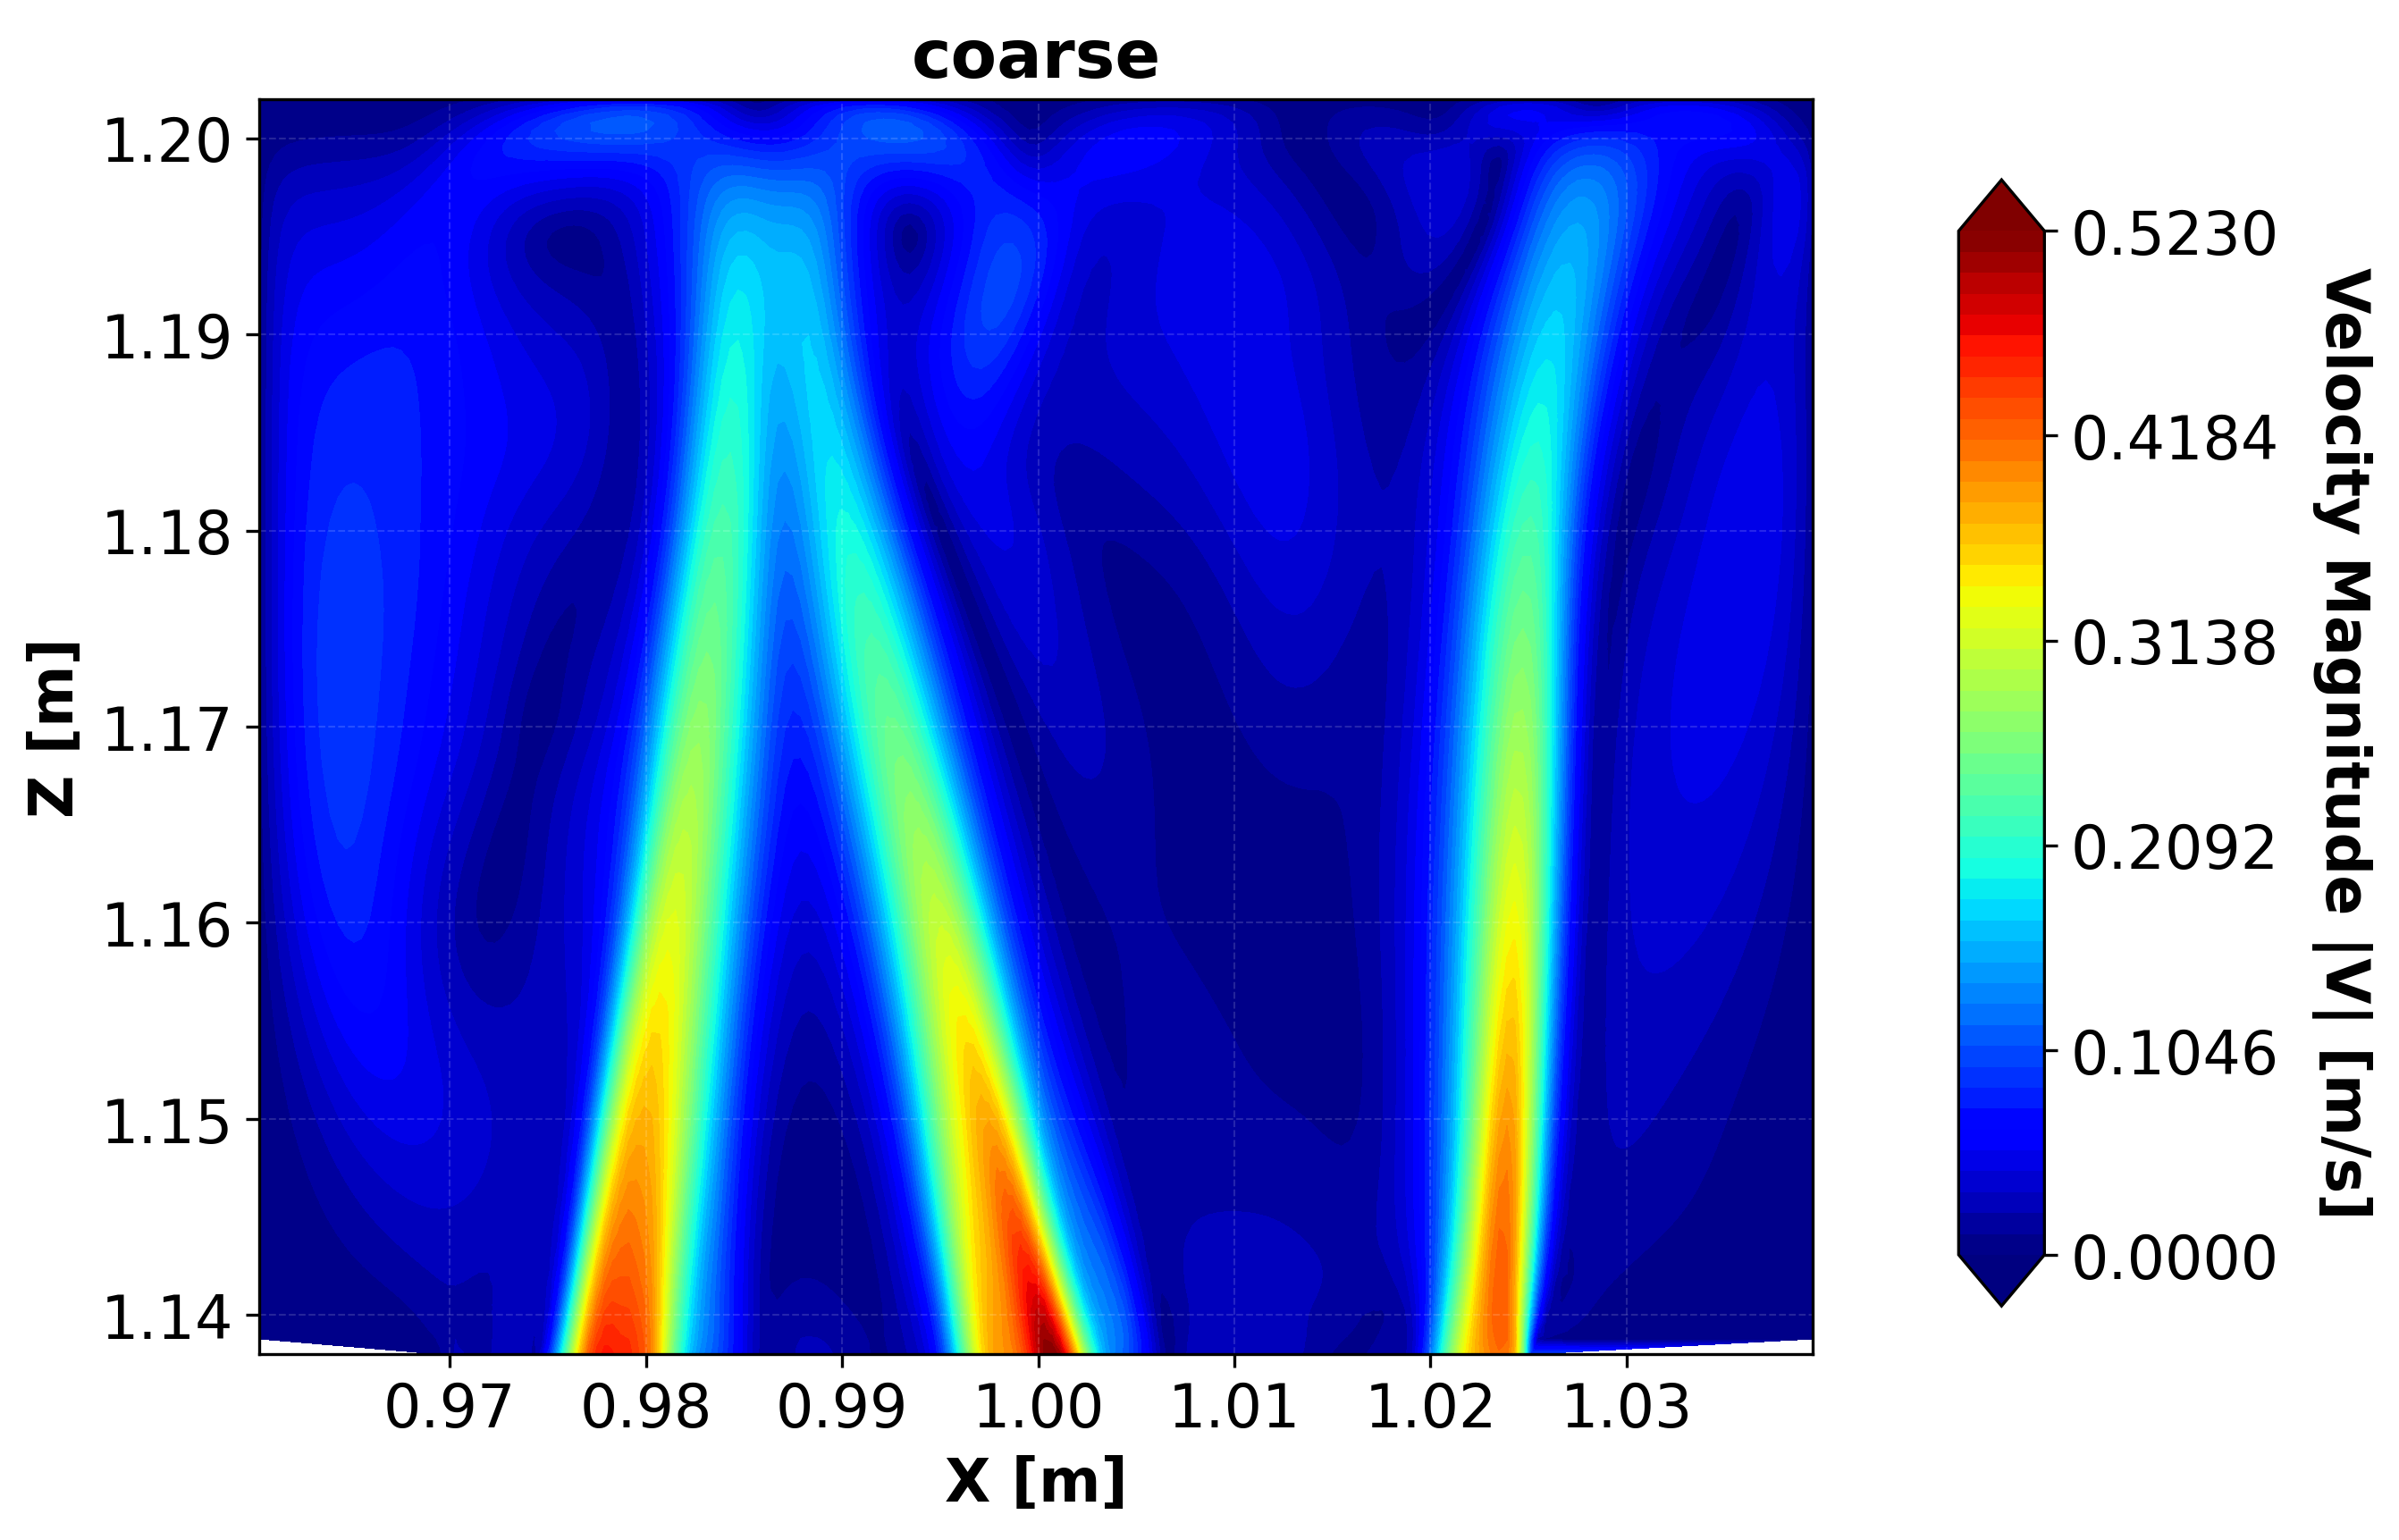
\includegraphics[width=0.32\textwidth]{grid_coarse.png}}\hfill
\subfloat[Medium]{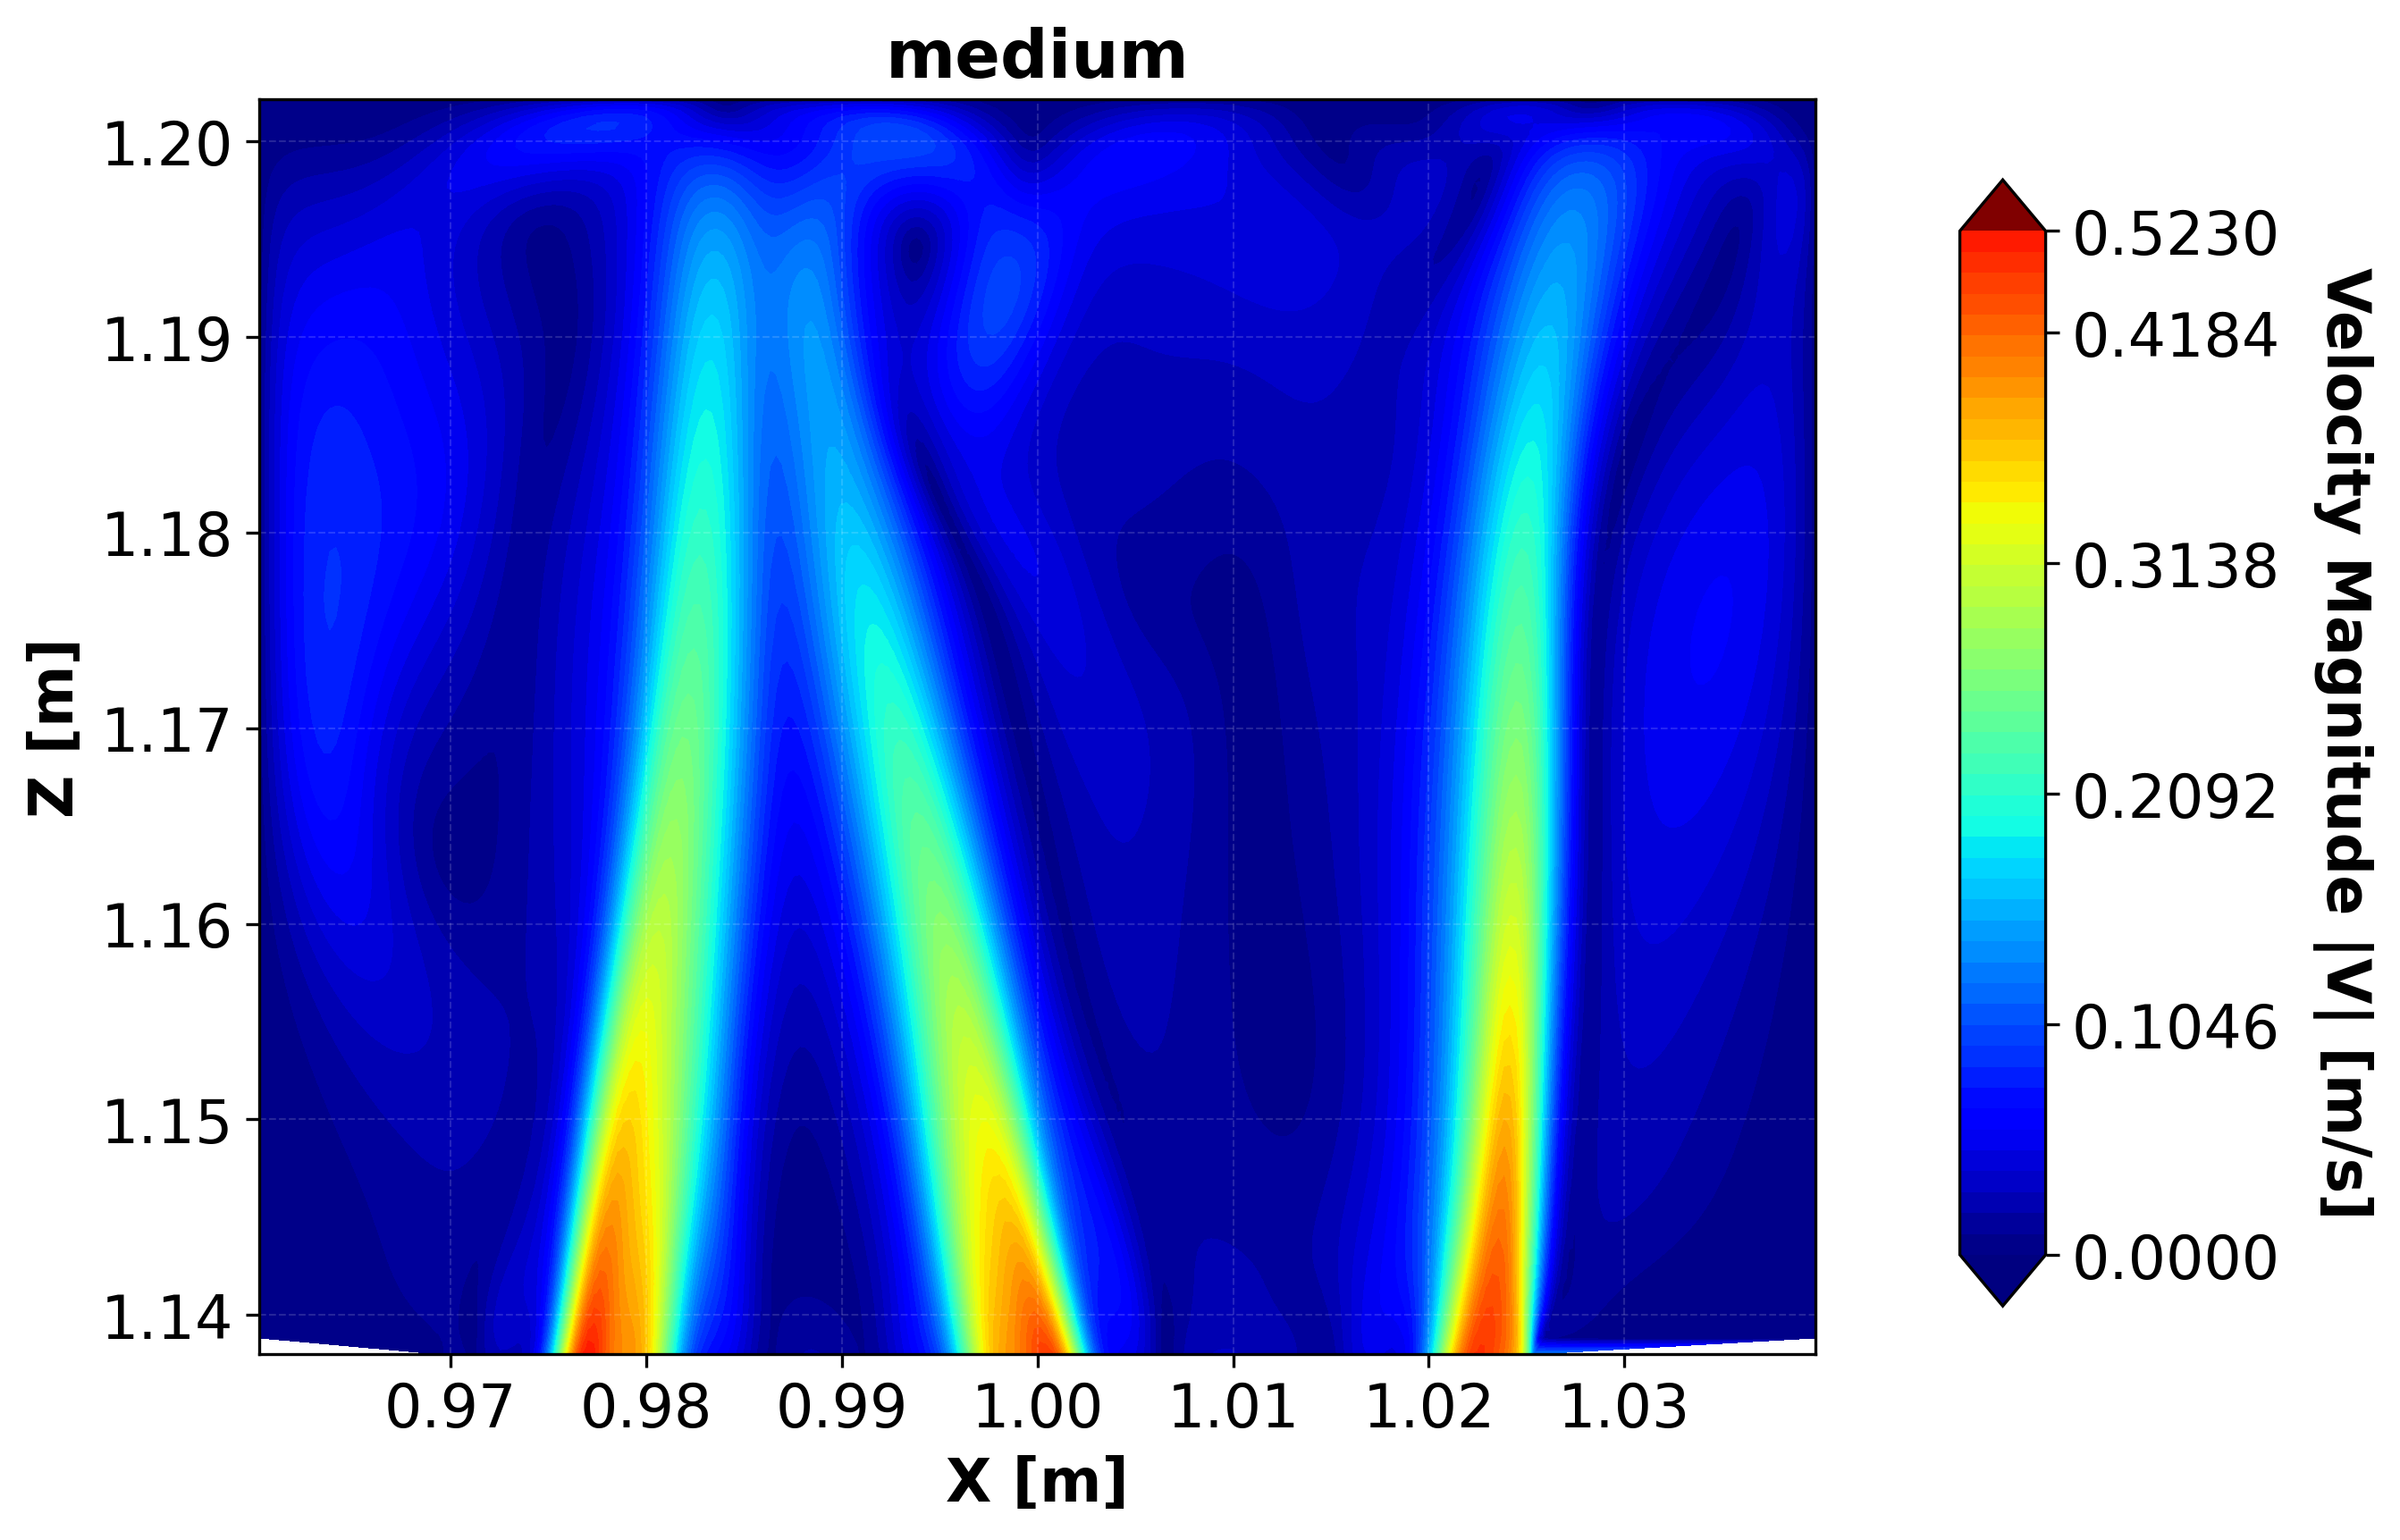
\includegraphics[width=0.32\textwidth]{grid_medium.png}}\hfill
\subfloat[Fine]{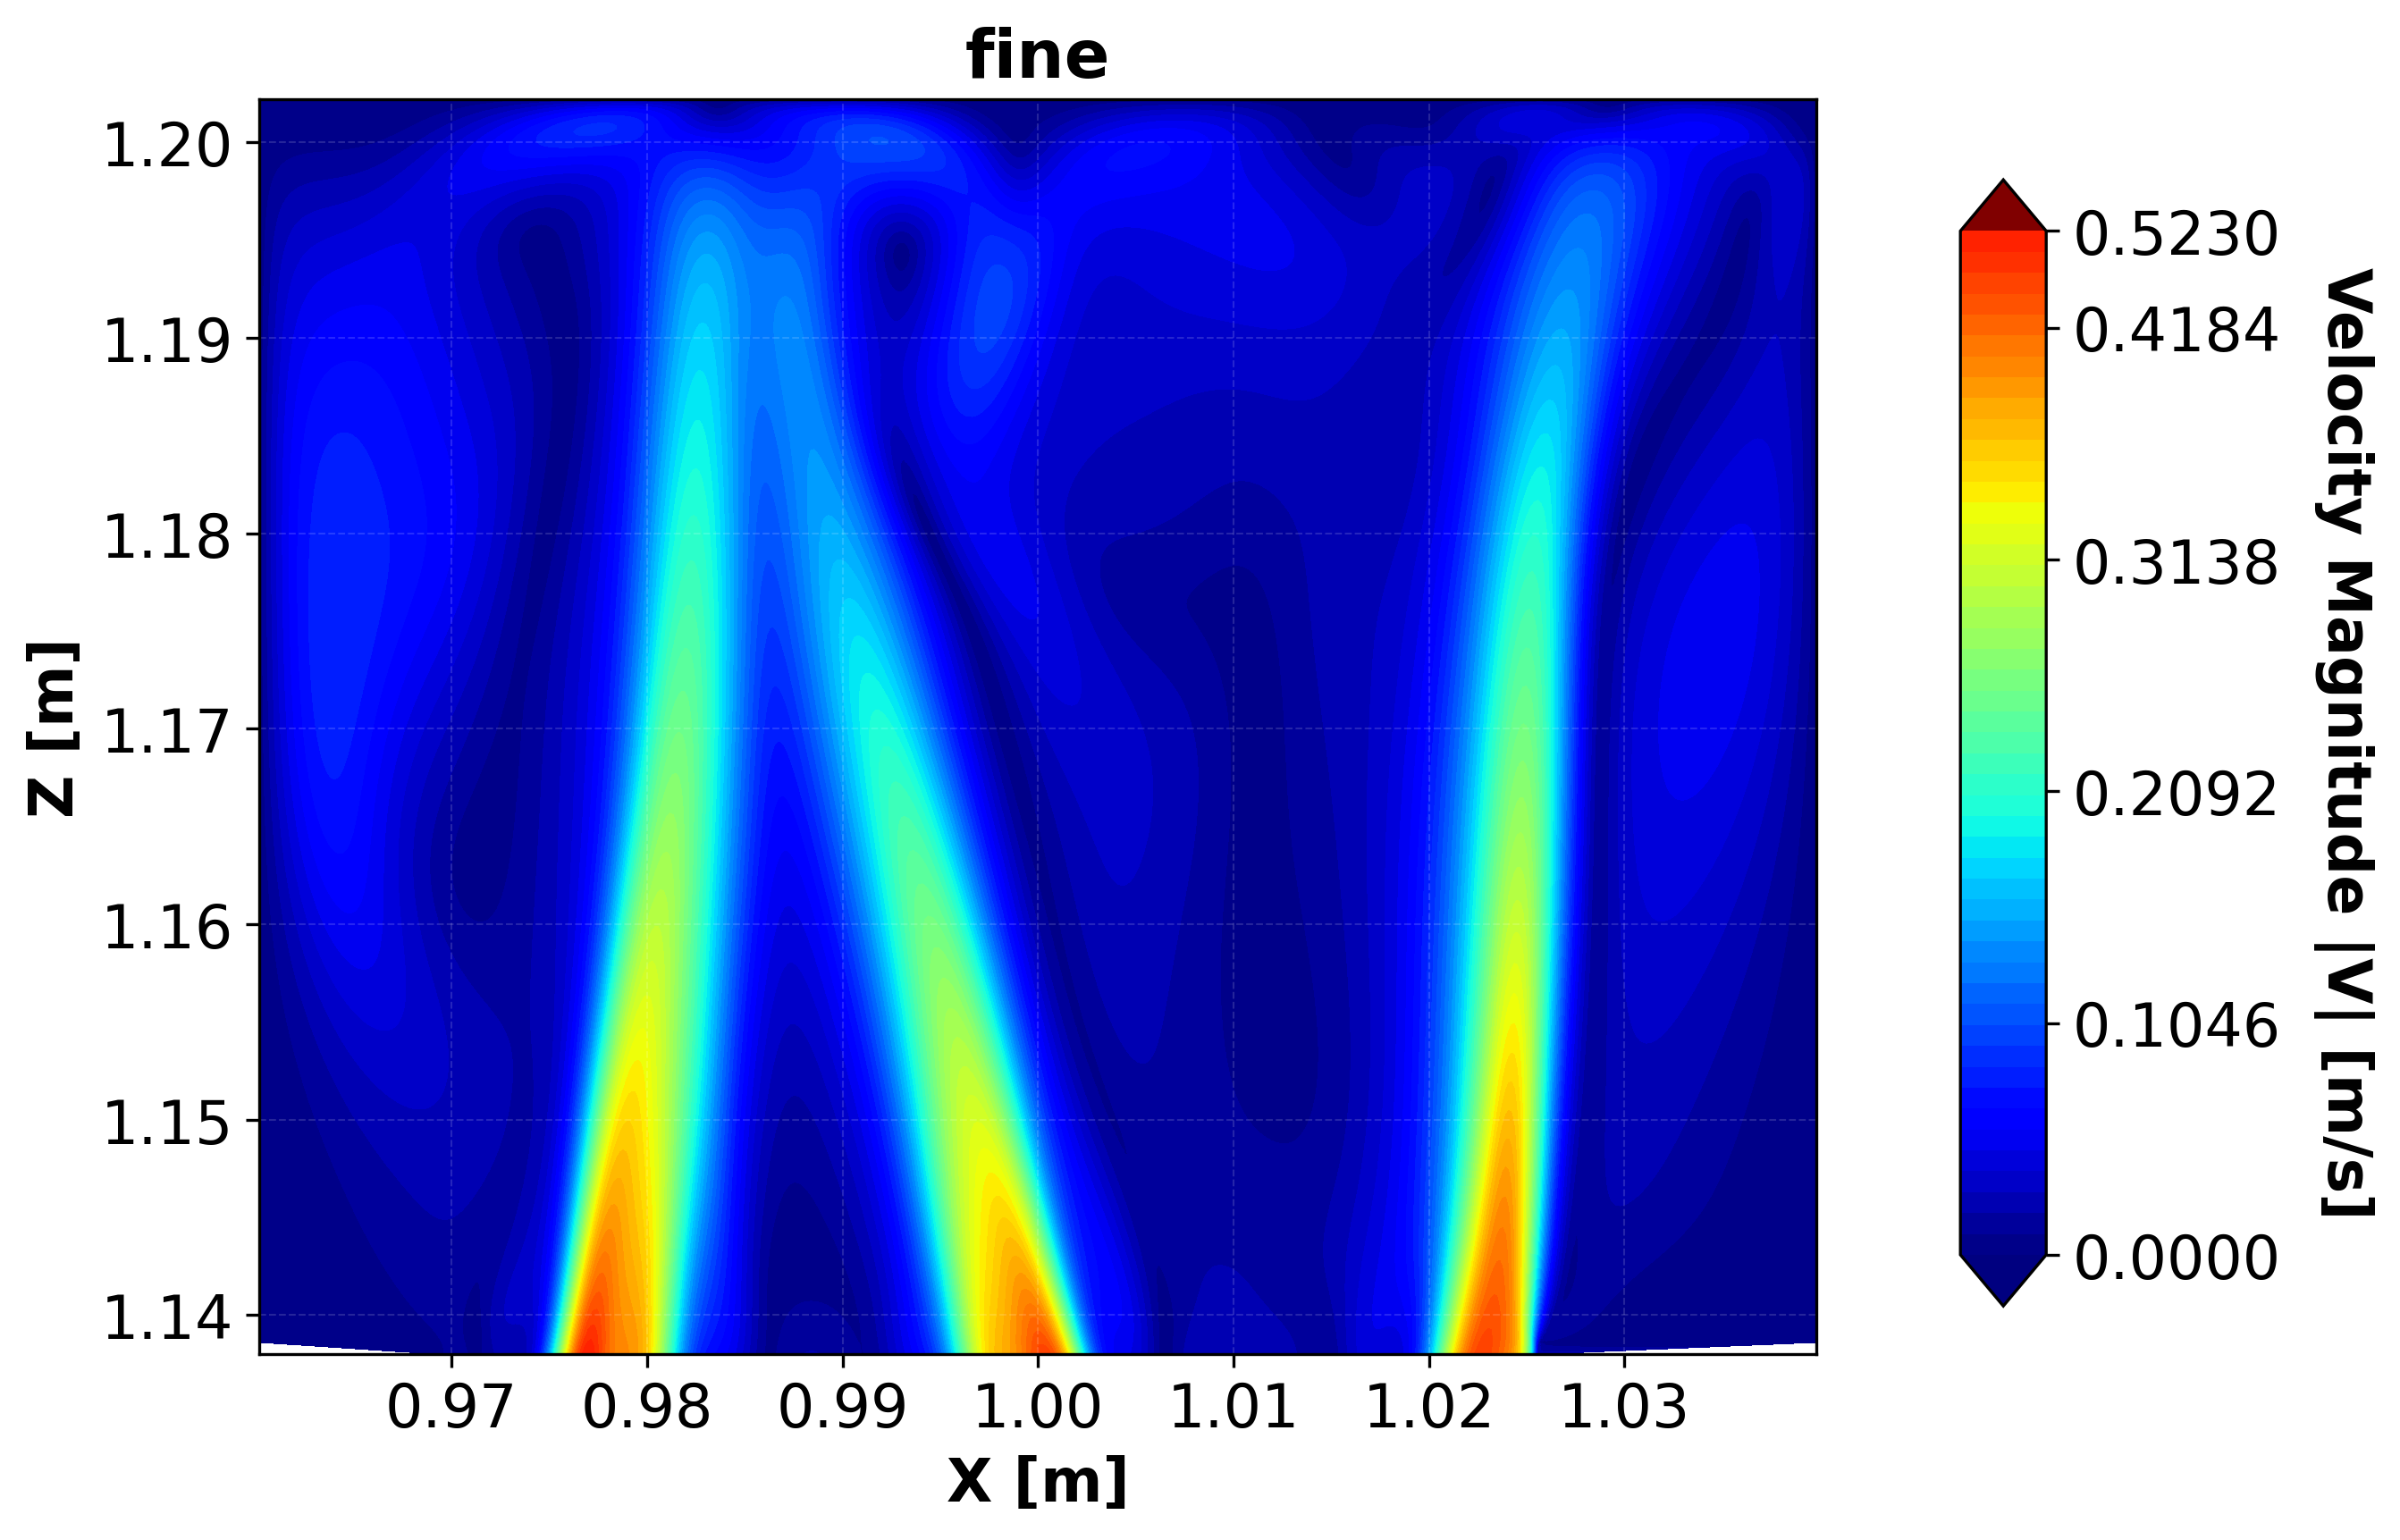
\includegraphics[width=0.32\textwidth]{grid_fine.png}}
\caption{Time-averaged velocity-magnitude field on a common extraction surface of the
$40^\circ$ subdomain for the three grid levels of Table~\ref{tab:grid}. The jet
structure is preserved across all resolutions; the medium and fine fields are nearly
identical.}
\label{fig:grid}
\end{figure}

The medium resolution was therefore adopted for the $Re_P = 100$ production runs as the
most efficient level meeting the convergence criterion. Relative to the fine grid it
carries roughly one third of the nodes and, through its four-times larger time step,
advances a given physical time at about an order of magnitude lower cost, while
reproducing the peak and integral flow quantities to better than a percent. The
higher-Reynolds-number cases ($Re_P = 300$ and $500$) are run on correspondingly finer
grids (Table~\ref{tab:simparams}) to keep the thinner shear layers resolved.

\subsection{Symmetry and Consistency Verification}
\label{sec:numerics:symmetry}

As an internal consistency check, the simulated flow should reproduce the point symmetry inherent to the slit arrangement. The measurement planes Pos,3 and Pos,5 are located at $a_\mathrm{Pos}=\mp7.5,\mathrm{mm}$ and form a point-symmetric pair about the column axis (Sec.~\ref{sec:geometry:coords}); consequently, their mean flow fields are expected to be mirror images of one another. Figure~\ref{fig:symmetry} compares the time-averaged velocity-magnitude contours and in-plane streamlines at these locations for the $30^\circ$ packing at $Re_P=100$ and $Re_P=300$. In both cases, the dominant flow features—including the central high-velocity jet, the adjacent slit jets, and the recirculation regions—are reproduced as near-perfect reflections across the two planes.
\begin{figure}[h]
\centering
\subfloat[$Re_P = 100$]{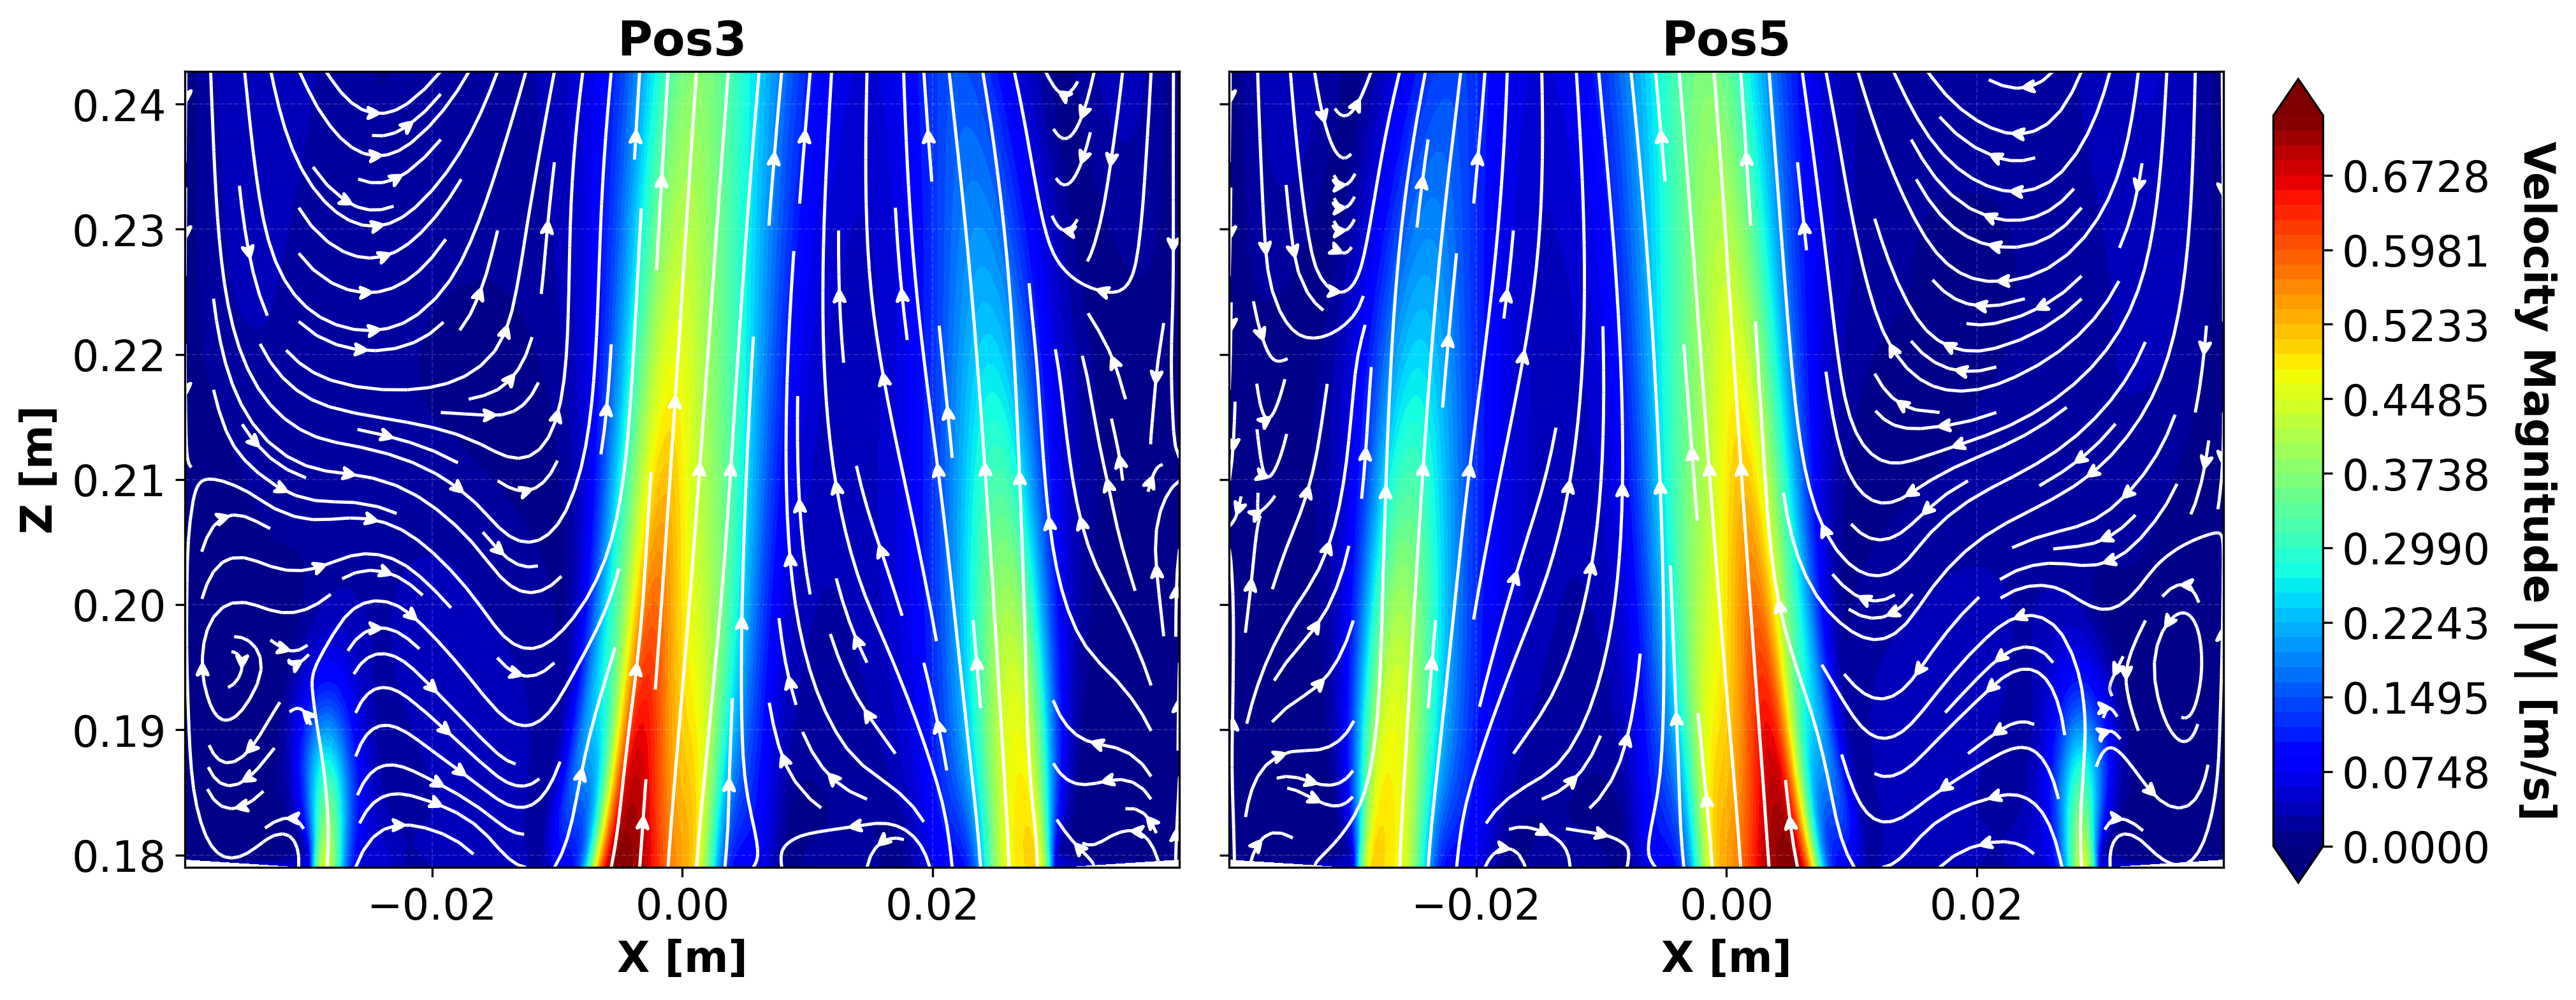
\includegraphics[width=0.9\linewidth]{Symmetry_Contour_Pos3_Re_100.png}}\\
\subfloat[$Re_P = 300$]{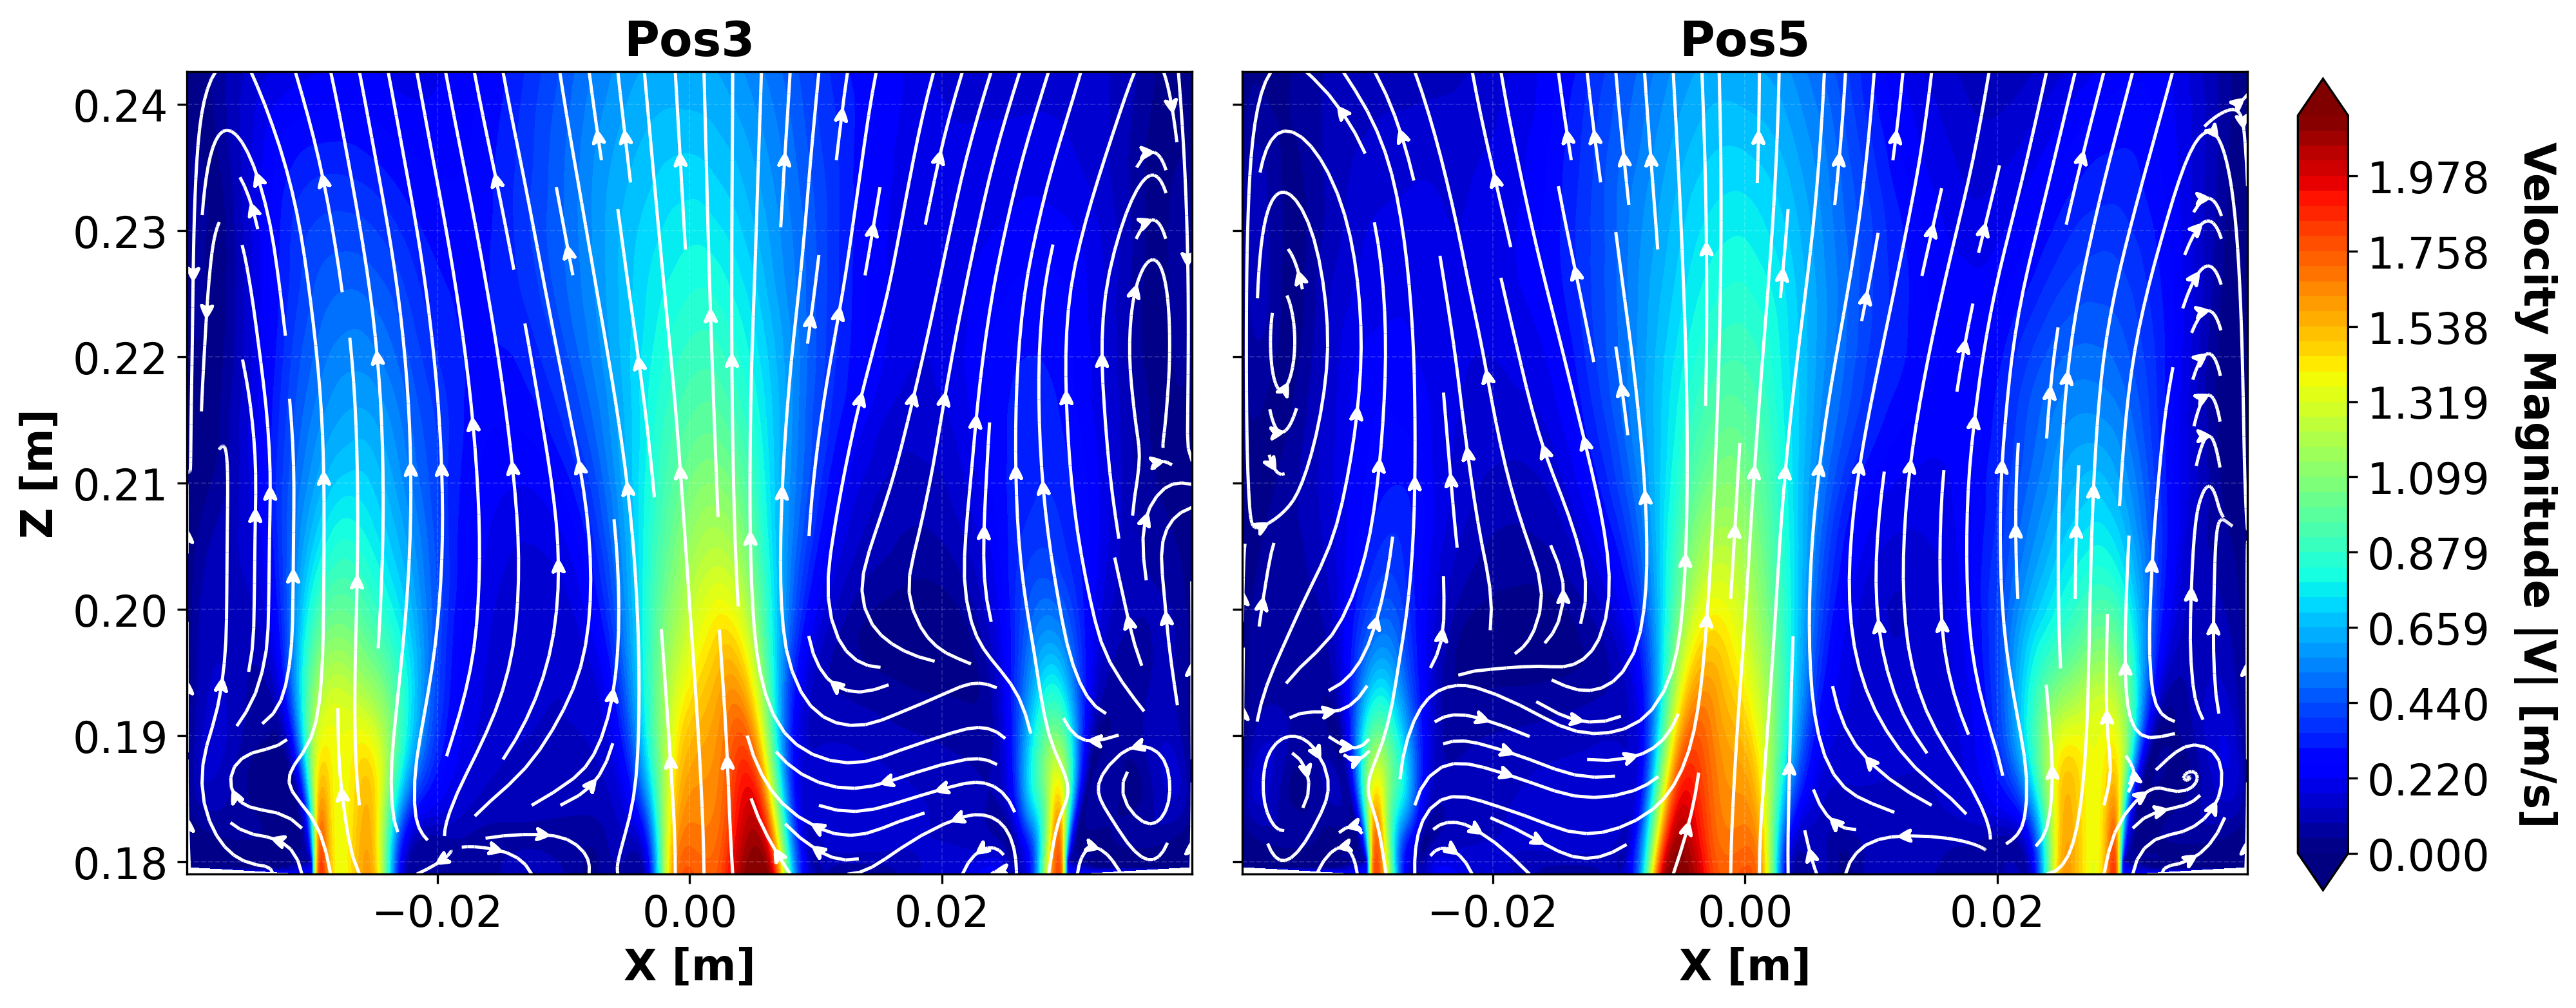
\includegraphics[width=0.9\linewidth]{Symmetry_Contour_Pos3_Re_300.png}}
\caption{Symmetry verification for the $30^\circ$ packing: time-averaged
velocity-magnitude contours with in-plane streamlines at the point-symmetric pair
Pos\,3 and Pos\,5, for (a)~$Re_P = 100$ and (b)~$Re_P = 300$. The Pos\,5 field is the
mirror image of Pos\,3 at both Reynolds numbers, verifying the $180^\circ$ symmetry of
the slit pattern.}
\label{fig:symmetry}
\end{figure}

\begin{figure}[h]
\centering
\subfloat[$Re_P = 100$]{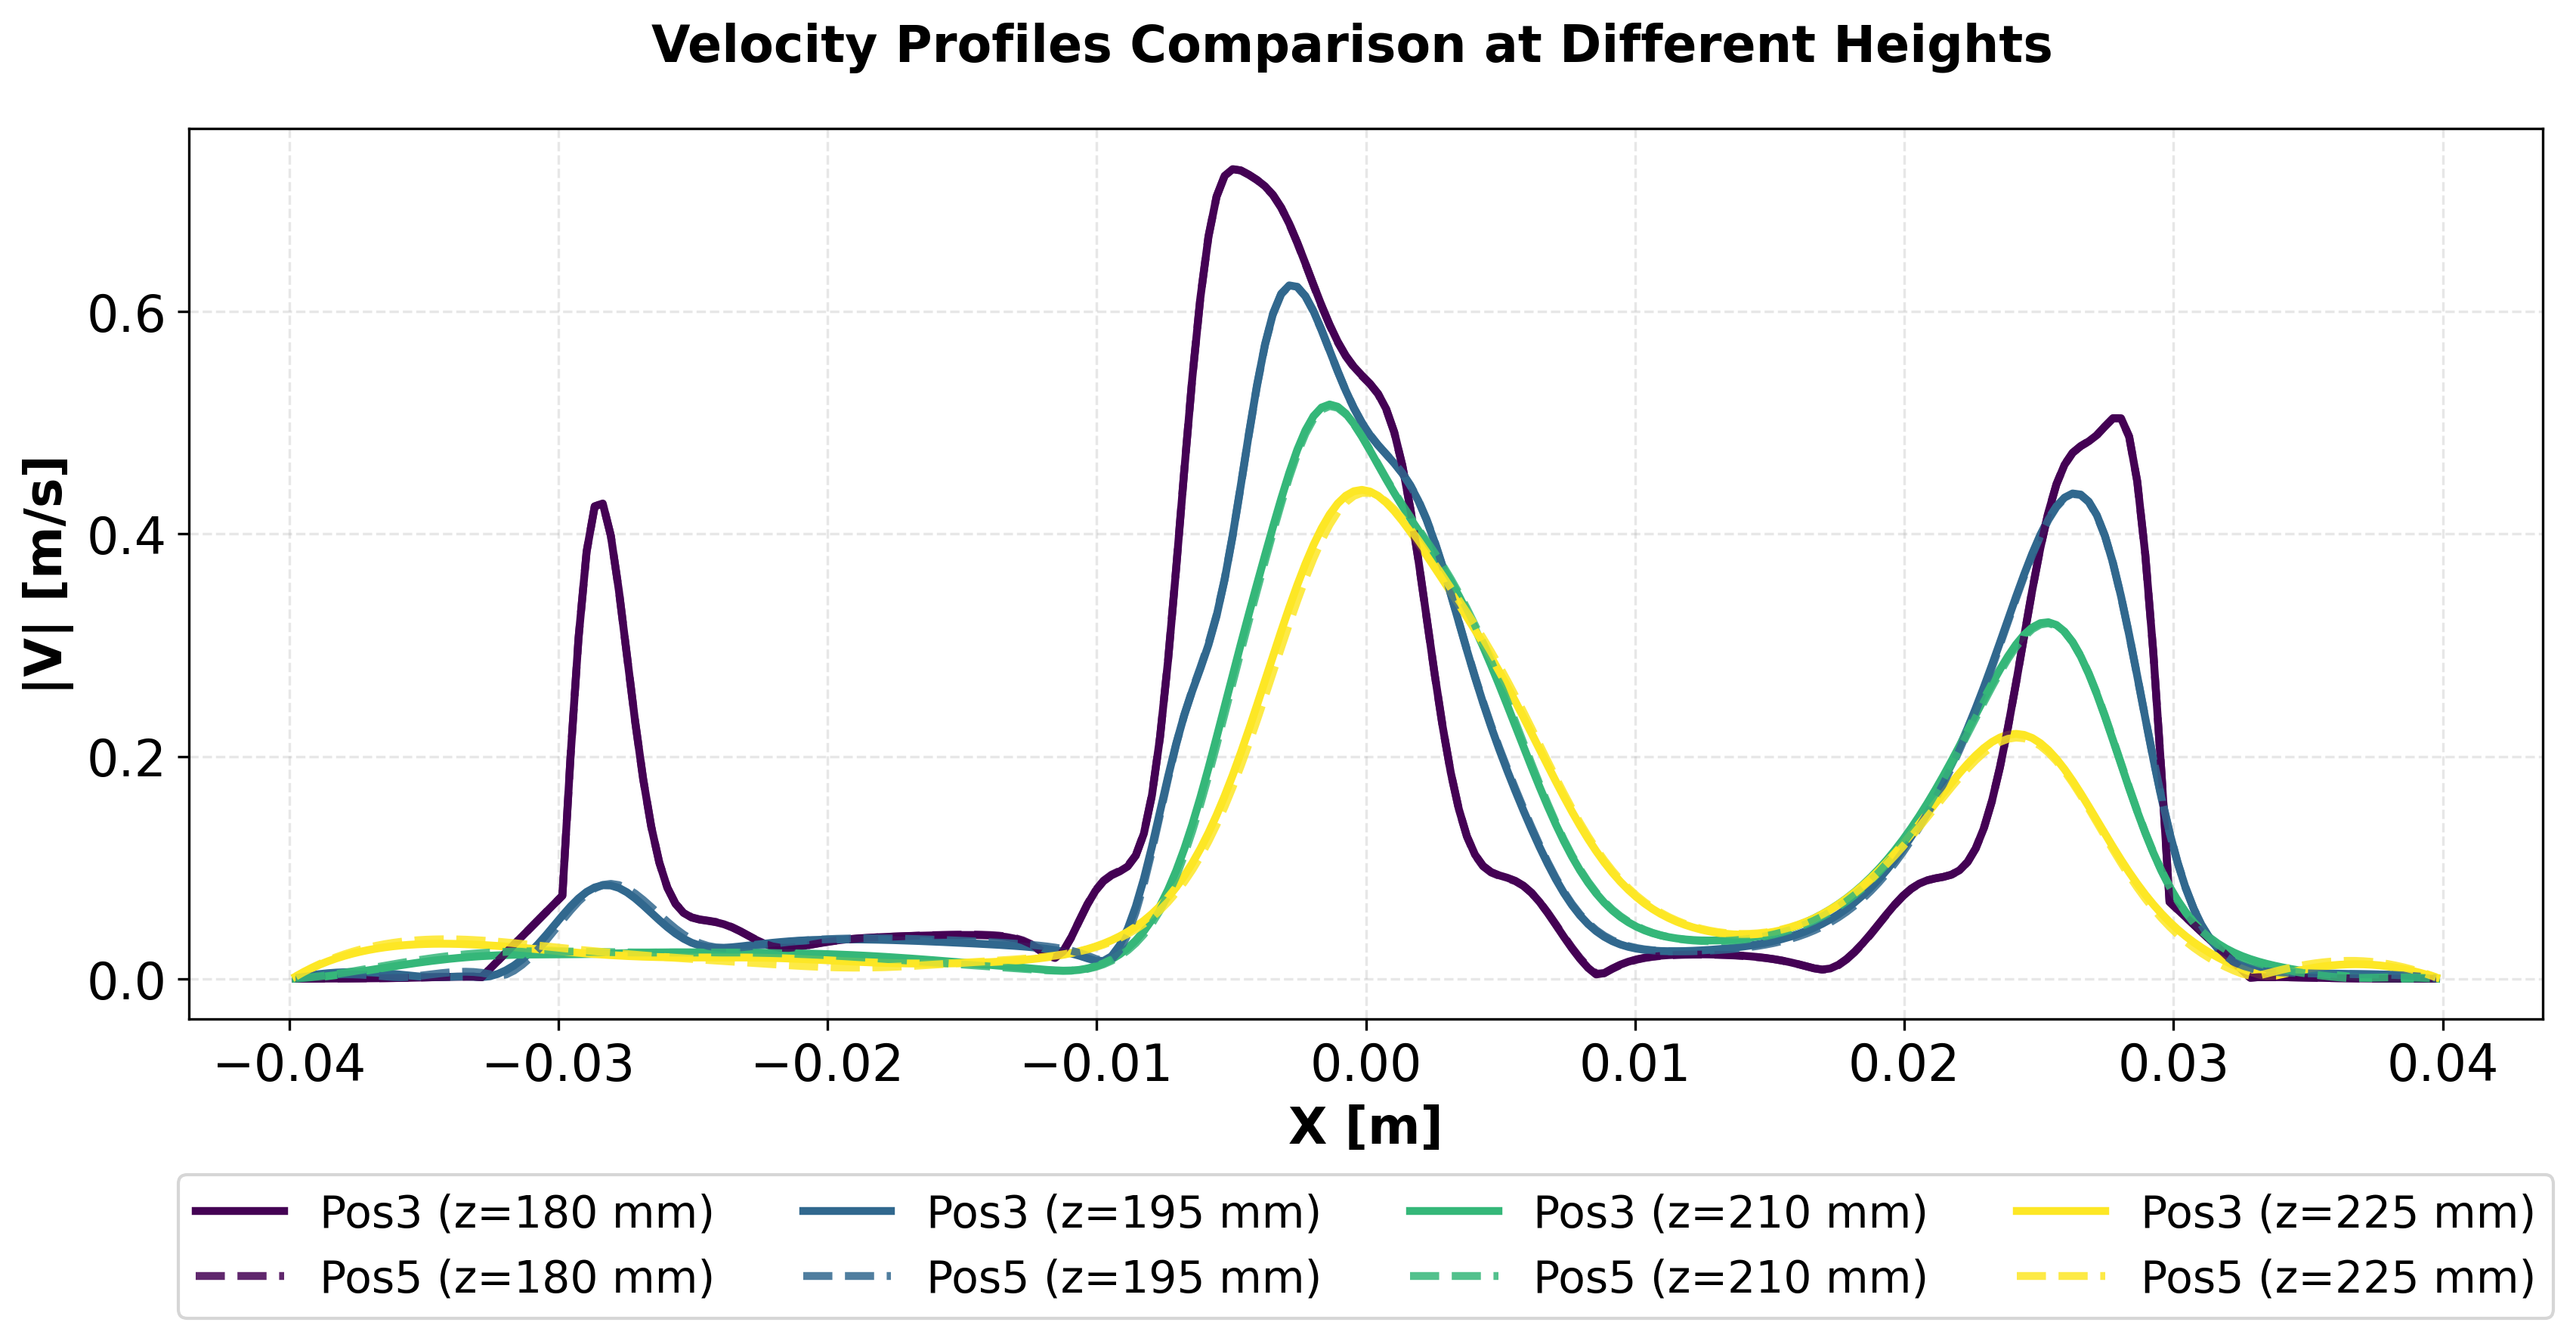
\includegraphics[width=0.9\linewidth]{Combined_Line_Profiles_Pos3_Re_100.png}}\\
\subfloat[$Re_P = 300$]{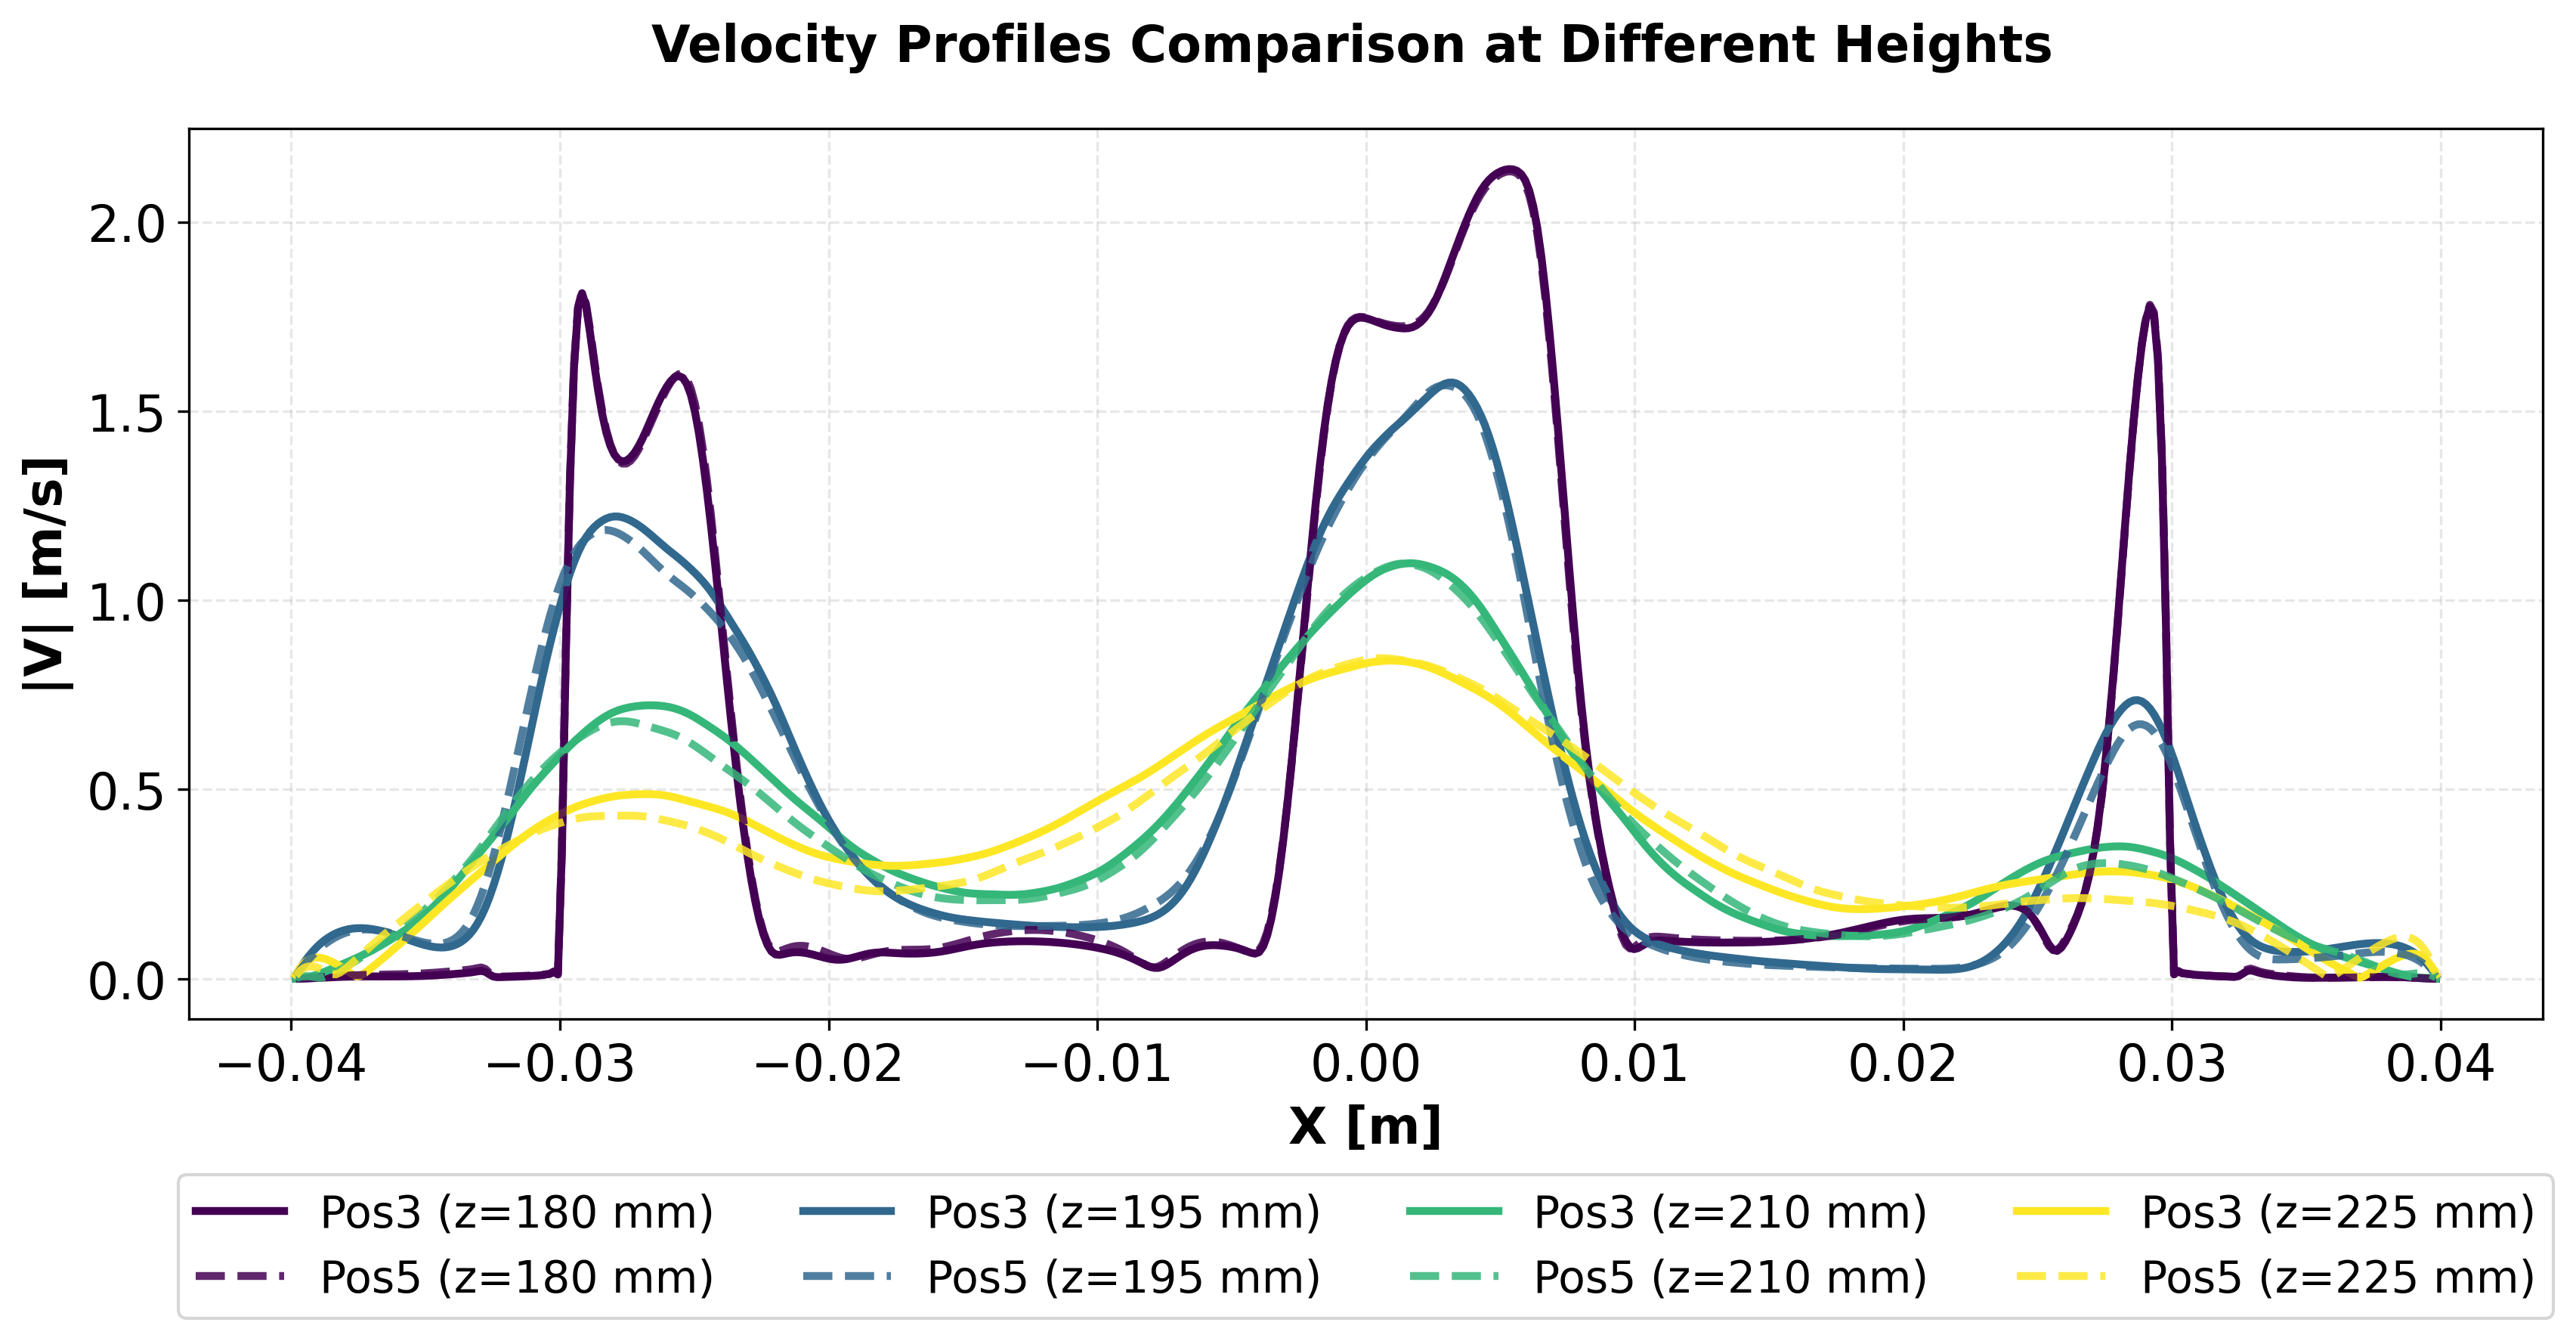
\includegraphics[width=0.9\linewidth]{Combined_Line_Profiles_Pos3_Re_300.png}}
\caption{Quantitative symmetry check: velocity-magnitude line profiles across the
plane at four streamwise heights, comparing Pos\,3 (solid) with its point-symmetric
partner Pos\,5 (dashed), for (a)~$Re_P = 100$ and (b)~$Re_P = 300$. The Pos\,3 and
Pos\,5 profiles coincide to within line width, confirming the $180^\circ$ symmetry of
the simulated mean flow.}
\label{fig:symmetry_profiles}
\end{figure}
The excellent agreement demonstrates that the numerical model preserves the geometric symmetry of the packing and, importantly, that the flow organisation remains point-symmetric over the investigated Reynolds-number range. This observation has a practical consequence for the validation procedure: because Pos,3 and Pos,5 contain equivalent flow information, detailed comparisons at one plane are representative of its symmetric counterpart. The symmetry therefore reduces the number of experimental measurement locations required from four to two without loss of information. To quantify this behaviour, Fig.~\ref{fig:symmetry_profiles} compares velocity-magnitude profiles at four streamwise heights. The profiles at Pos,3 and Pos,5 are virtually indistinguishable at both Reynolds numbers, confirming that the symmetry remains robust from $Re_P=100$ to $Re_P=300$.

%% ============================================================
\section{Validation against PIV Measurements}
\label{sec:validation}

The simulations are validated against the published PIV data
of~\citet{velten2026} for all three topologies. This section first defines the
comparison procedure and the error metrics, then assesses the time-averaged
velocity-magnitude fields over the measurement planes (surface validation); the
layer-resolved development of the flow within the slits is examined subsequently.

\subsection{Comparison Procedure and Error Metrics}
\label{sec:validation:procedure}

Velocity data are reported in the in-plane coordinate system of~\citet{velten2026}:
the horizontal in-plane axis $\xi$ and the vertical streamwise axis $z$.
Simulation planes are extracted at the physical positions corresponding to Pos\,1 and
Pos\,3 ($a_\mathrm{Pos} = -22.5$ and $-7.5\,\mathrm{mm}$ from the reactor centre);
the two remaining measurement positions, Pos\,5 and Pos\,7, are point-symmetric
partners of Pos\,3 and Pos\,1 (Sec.~\ref{sec:numerics:symmetry}) and therefore carry
no additional information.
Each extracted plane is masked to the fluid region, interpolated onto the experimental
PIV grid (vector resolution $3.40$-$3.44\,\mathrm{vec/mm}$, Table~2 of
\citealt{velten2026}), and compared with the measured field point by point.

Agreement is quantified on the velocity magnitude $|\bm{v}|$ over all $M$ fluid grid
points of a plane. Denoting the simulated and experimental values at point $i$ by
$s_i$ and $e_i$, we report the root-mean-square error
\begin{equation}
    \mathrm{RMSE} = \sqrt{\frac{1}{M}\sum_{i=1}^{M}\left(s_i-e_i\right)^2},
    \qquad
    \mathrm{NRMSE} = \frac{\mathrm{RMSE}}{e_\mathrm{max}-e_\mathrm{min}},
    \label{eq:rmse}
\end{equation}
its value normalised by the experimental dynamic range ($\mathrm{NRMSE}$), the mean
signed deviation, or bias, $\overline{s-e}$, and the coefficient of determination
$R^2 = 1-\sum_i(s_i-e_i)^2/\sum_i(e_i-\bar{e})^2$, which measures how much of the
spatial variance of the measured field is reproduced. $\mathrm{NRMSE}$ is the primary
headline metric, as it is insensitive to the absolute velocity level and is therefore
comparable across topologies and Reynolds numbers.

\subsection{Surface Velocity Fields}
\label{sec:validation:surface}

Figure~\ref{fig:validation_surface} compares the time-averaged velocity-magnitude
fields and in-plane streamlines, simulation versus PIV, for the $30^\circ$ packing at
$Re_P=100$ at the two independent positions Pos\,1 and Pos\,3. The flow over the
measurement window is organised into discrete streamwise jets issuing from the slits,
separated by low-velocity wakes behind the bars; at Pos\,3 a strong central jet at
$x\approx0$ is flanked by weaker slit jets, while Pos\,1 samples the more uniform
near-edge region. The simulation reproduces the number, position, width, and peak
magnitude of these jets, as well as the streamline topology of the intervening
recirculation zones.

The agreement is quantified in Fig.~\ref{fig:validation_profiles}, which overlays
velocity-magnitude profiles across the plane at four streamwise heights
($z=183$-$213\,\mathrm{mm}$) for Pos\,3, together with the experimental uncertainty
band. The simulated profiles fall within or close to the measured band almost
everywhere; the jet peaks and the inter-jet minima are captured, and the residual
deviations are confined to the steep shear layers bordering the central jet, where
sub-vector-spacing velocity gradients and PIV peak-locking are largest.

Global error metrics for all cases and positions are collected in
Table~\ref{tab:validation}. For the two regular packings the simulation reproduces the
measured fields to within $\mathrm{NRMSE}=5$-$9\%$ with coefficients of determination
$R^2=0.75$-$0.93$ and a near-zero bias, and this level of agreement is maintained at
the higher Reynolds number ($30^\circ$, $Re_P=300$), confirming that the model remains
predictive as the flow strengthens. The error is spatially concentrated in the
high-gradient jet shear layers (local-error maps, Supplementary Material), while the
bulk of each plane agrees to within a few percent; the slightly larger $\mathrm{NRMSE}$
at Pos\,1 reflects the lower velocity range there, which makes the normalisation more
sensitive rather than indicating a genuine loss of accuracy.

The irregular packing is reproduced less tightly: while Pos\,1 still attains
$\mathrm{NRMSE}=7.5\%$, the coefficient of determination at Pos\,3 falls to $R^2=0.10$
at $\mathrm{NRMSE}=11.7\%$. The aperiodic arrangement produces a spatially disordered
field with a comparatively small dynamic range, so a point-by-point metric such as
$R^2$ becomes stringent and is highly sensitive to the exact bar placement; the overall
magnitude and the jet/wake distribution are nonetheless captured to within
$\approx 12\%$. This contrast---reproducible, low-error fields for the periodic
packings versus a looser, placement-sensitive match for the irregular one---already
foreshadows the flow-locking analysis of Sec.~\ref{sec:locking}.

\begin{table}[h]
\centering
\caption{Surface-field validation against PIV: global error metrics for the
time-averaged velocity magnitude over the measurement planes. $\mathrm{NRMSE}$ is
normalised by the experimental dynamic range; bias is the mean signed deviation
$\overline{s-e}$.}
\label{tab:validation}
\begin{tabular}{llccc}
\hline\noalign{\smallskip}
Packing & $Re_P$ & Position & $\mathrm{NRMSE}$ (\%) & $R^2$ \\
\noalign{\smallskip}\hline\noalign{\smallskip}
$30^\circ$        & 100 & Pos\,1 & 9.4  & 0.75 \\
$30^\circ$        & 100 & Pos\,3 & 5.7  & 0.92 \\
$30^\circ$        & 300 & Pos\,1 & 5.6  & 0.86 \\
$30^\circ$        & 300 & Pos\,3 & 5.1  & 0.93 \\
$40^\circ$        & 100 & Pos\,1 & 9.0  & 0.83 \\
$40^\circ$        & 100 & Pos\,3 & 7.7  & 0.88 \\
Irregular         & 100 & Pos\,1 & 7.5  & 0.67 \\
Irregular         & 100 & Pos\,3 & 11.7 & 0.10 \\
\noalign{\smallskip}\hline
\end{tabular}
\end{table}

\begin{figure}[h]
\centering
\subfloat[Pos\,1]{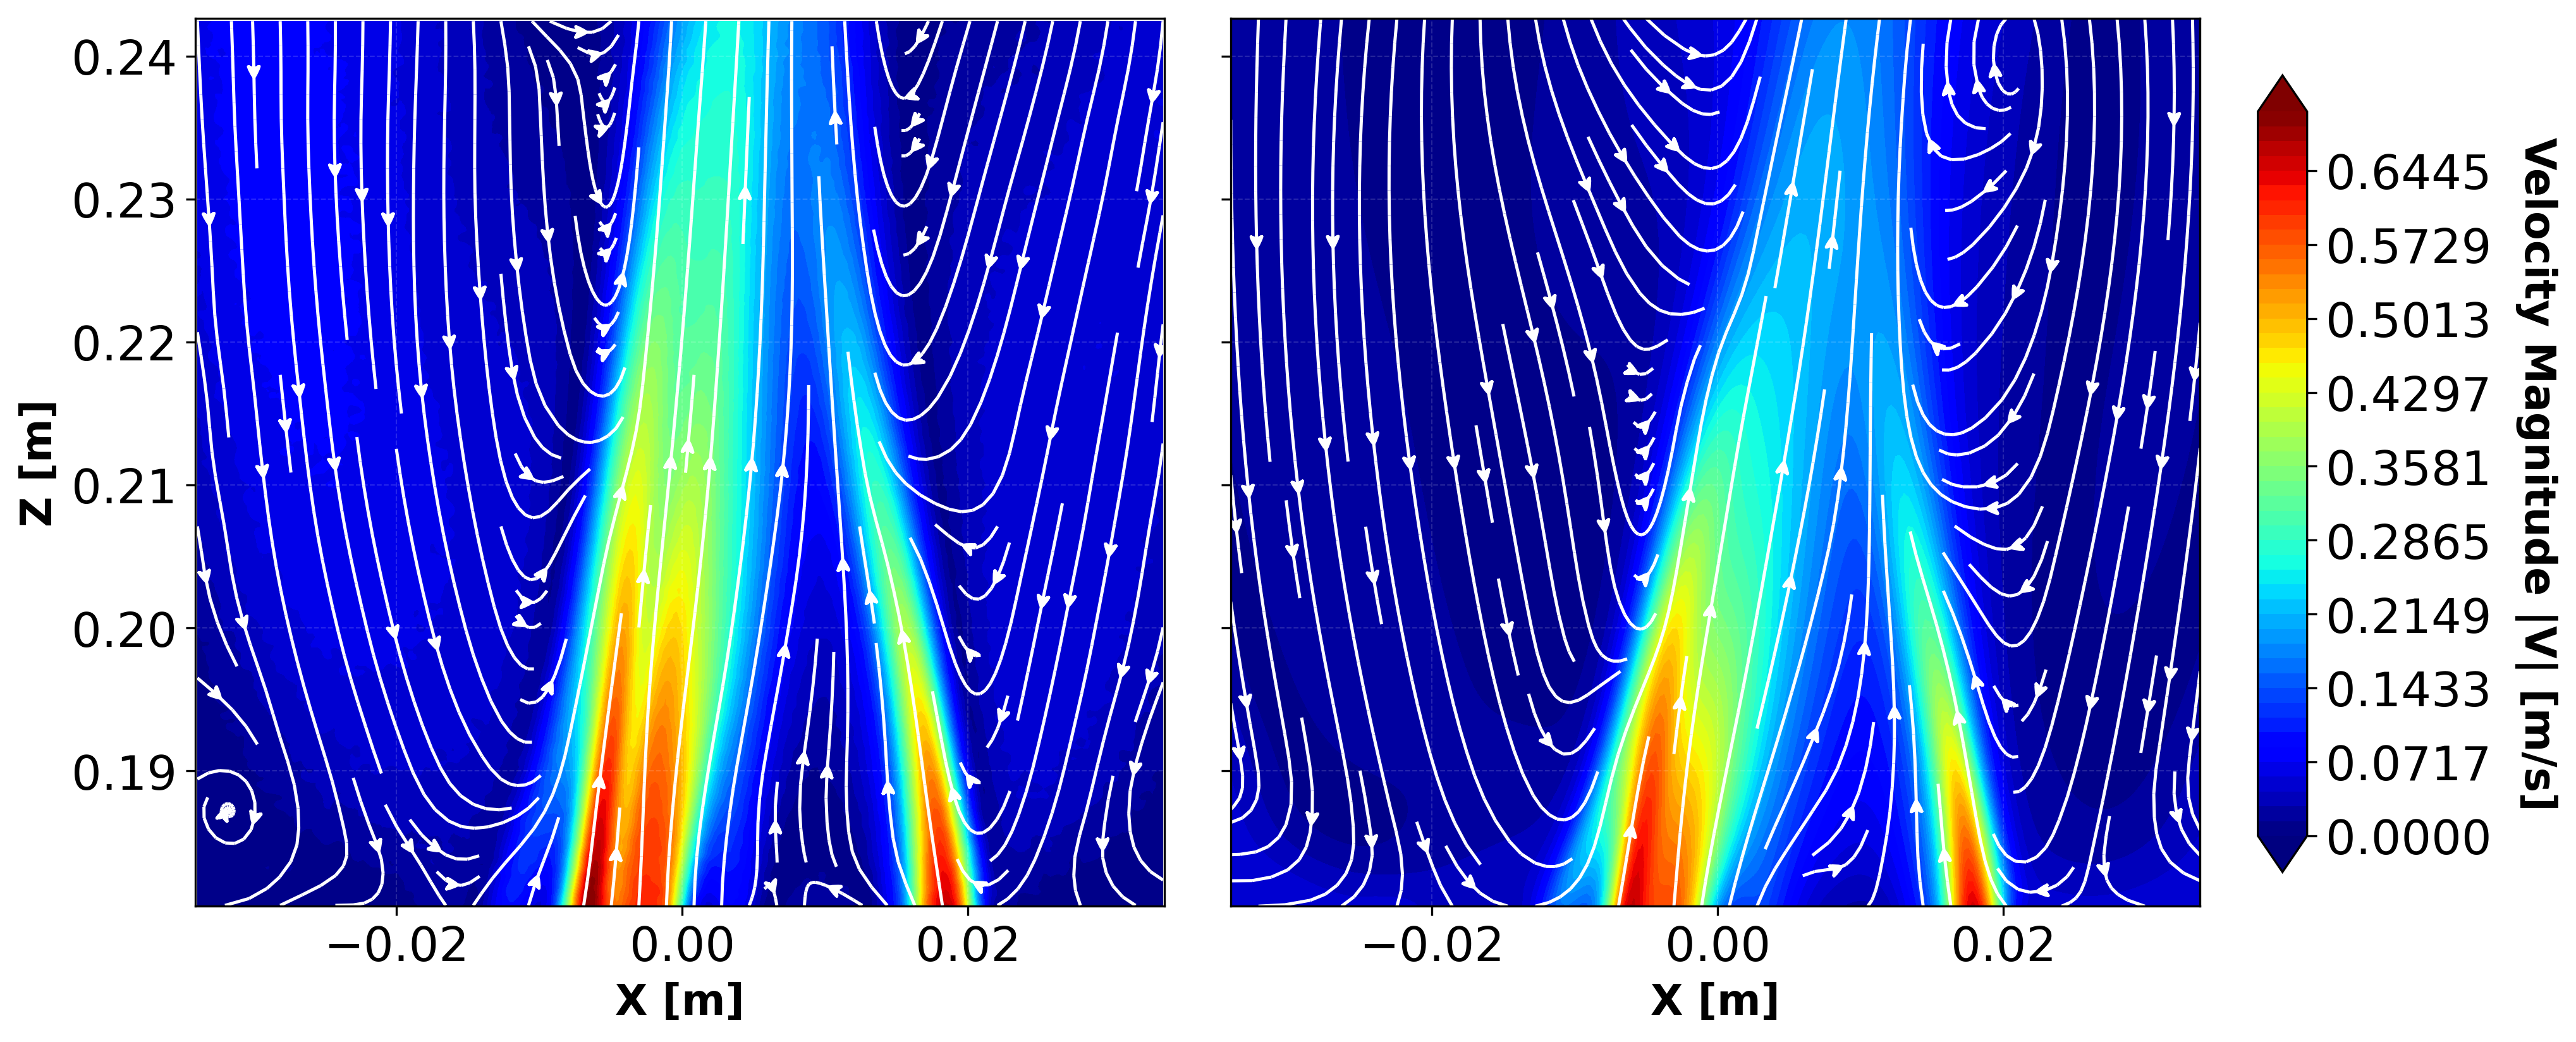
\includegraphics[width=0.48\linewidth]{30_Re_100/surface/pos1_Surface_plot.png}}\hfill
\subfloat[Pos\,3]{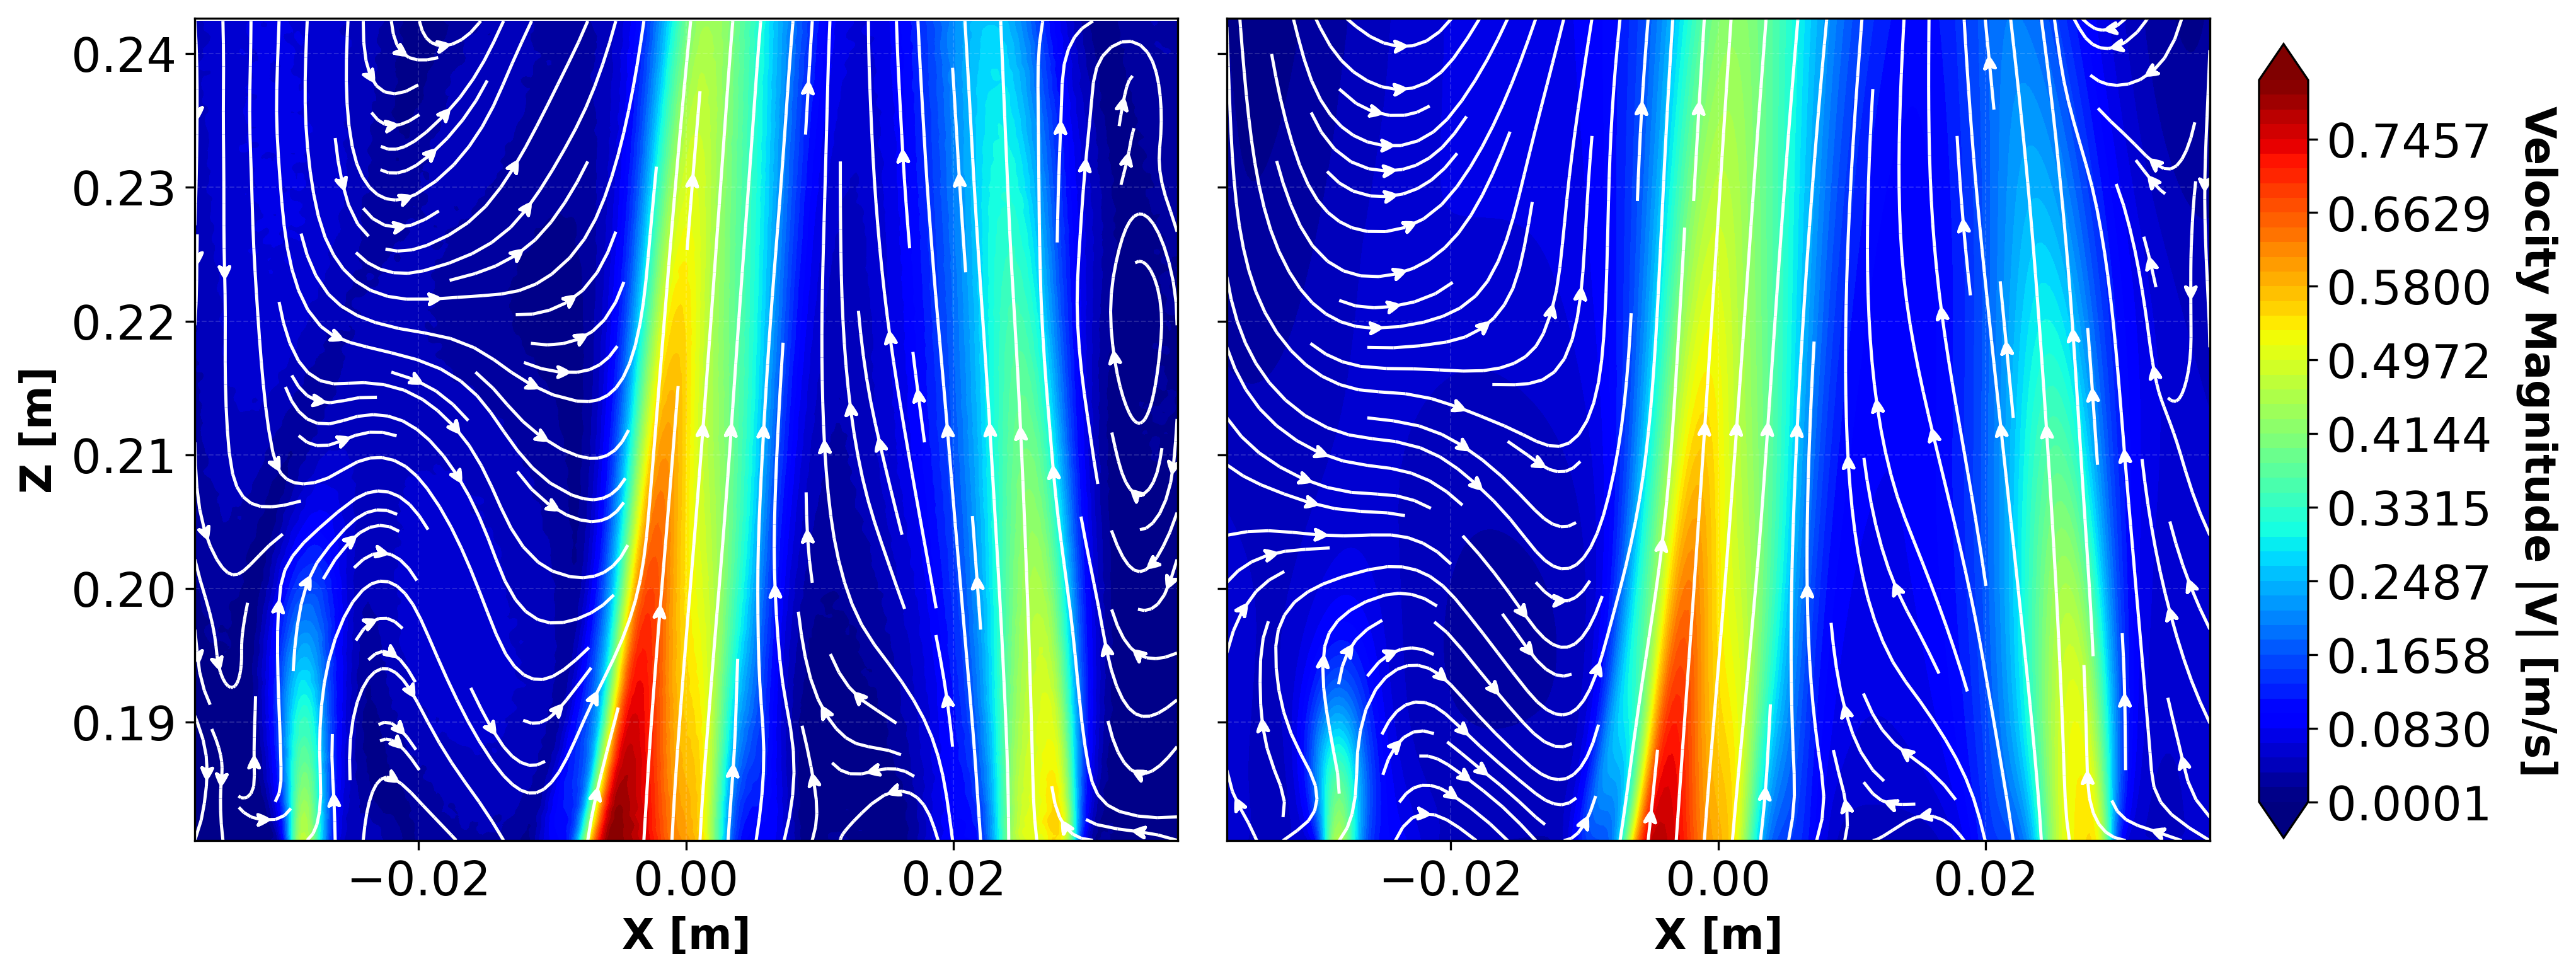
\includegraphics[width=0.48\linewidth]{30_Re_100/surface/pos3_Surface_plot.png}}
\caption{Surface validation for the $30^\circ$ packing at $Re_P=100$: time-averaged
velocity-magnitude fields with in-plane streamlines, simulation (left of each pair)
versus experiment (right), at the two independent measurement positions
(a)~Pos\,1 and (b)~Pos\,3 over layers L13-L17. The simulation reproduces the position,
width, and strength of the slit jets and the intervening recirculation pattern.}
\label{fig:validation_surface}
\end{figure}

\begin{figure}[h]
\centering
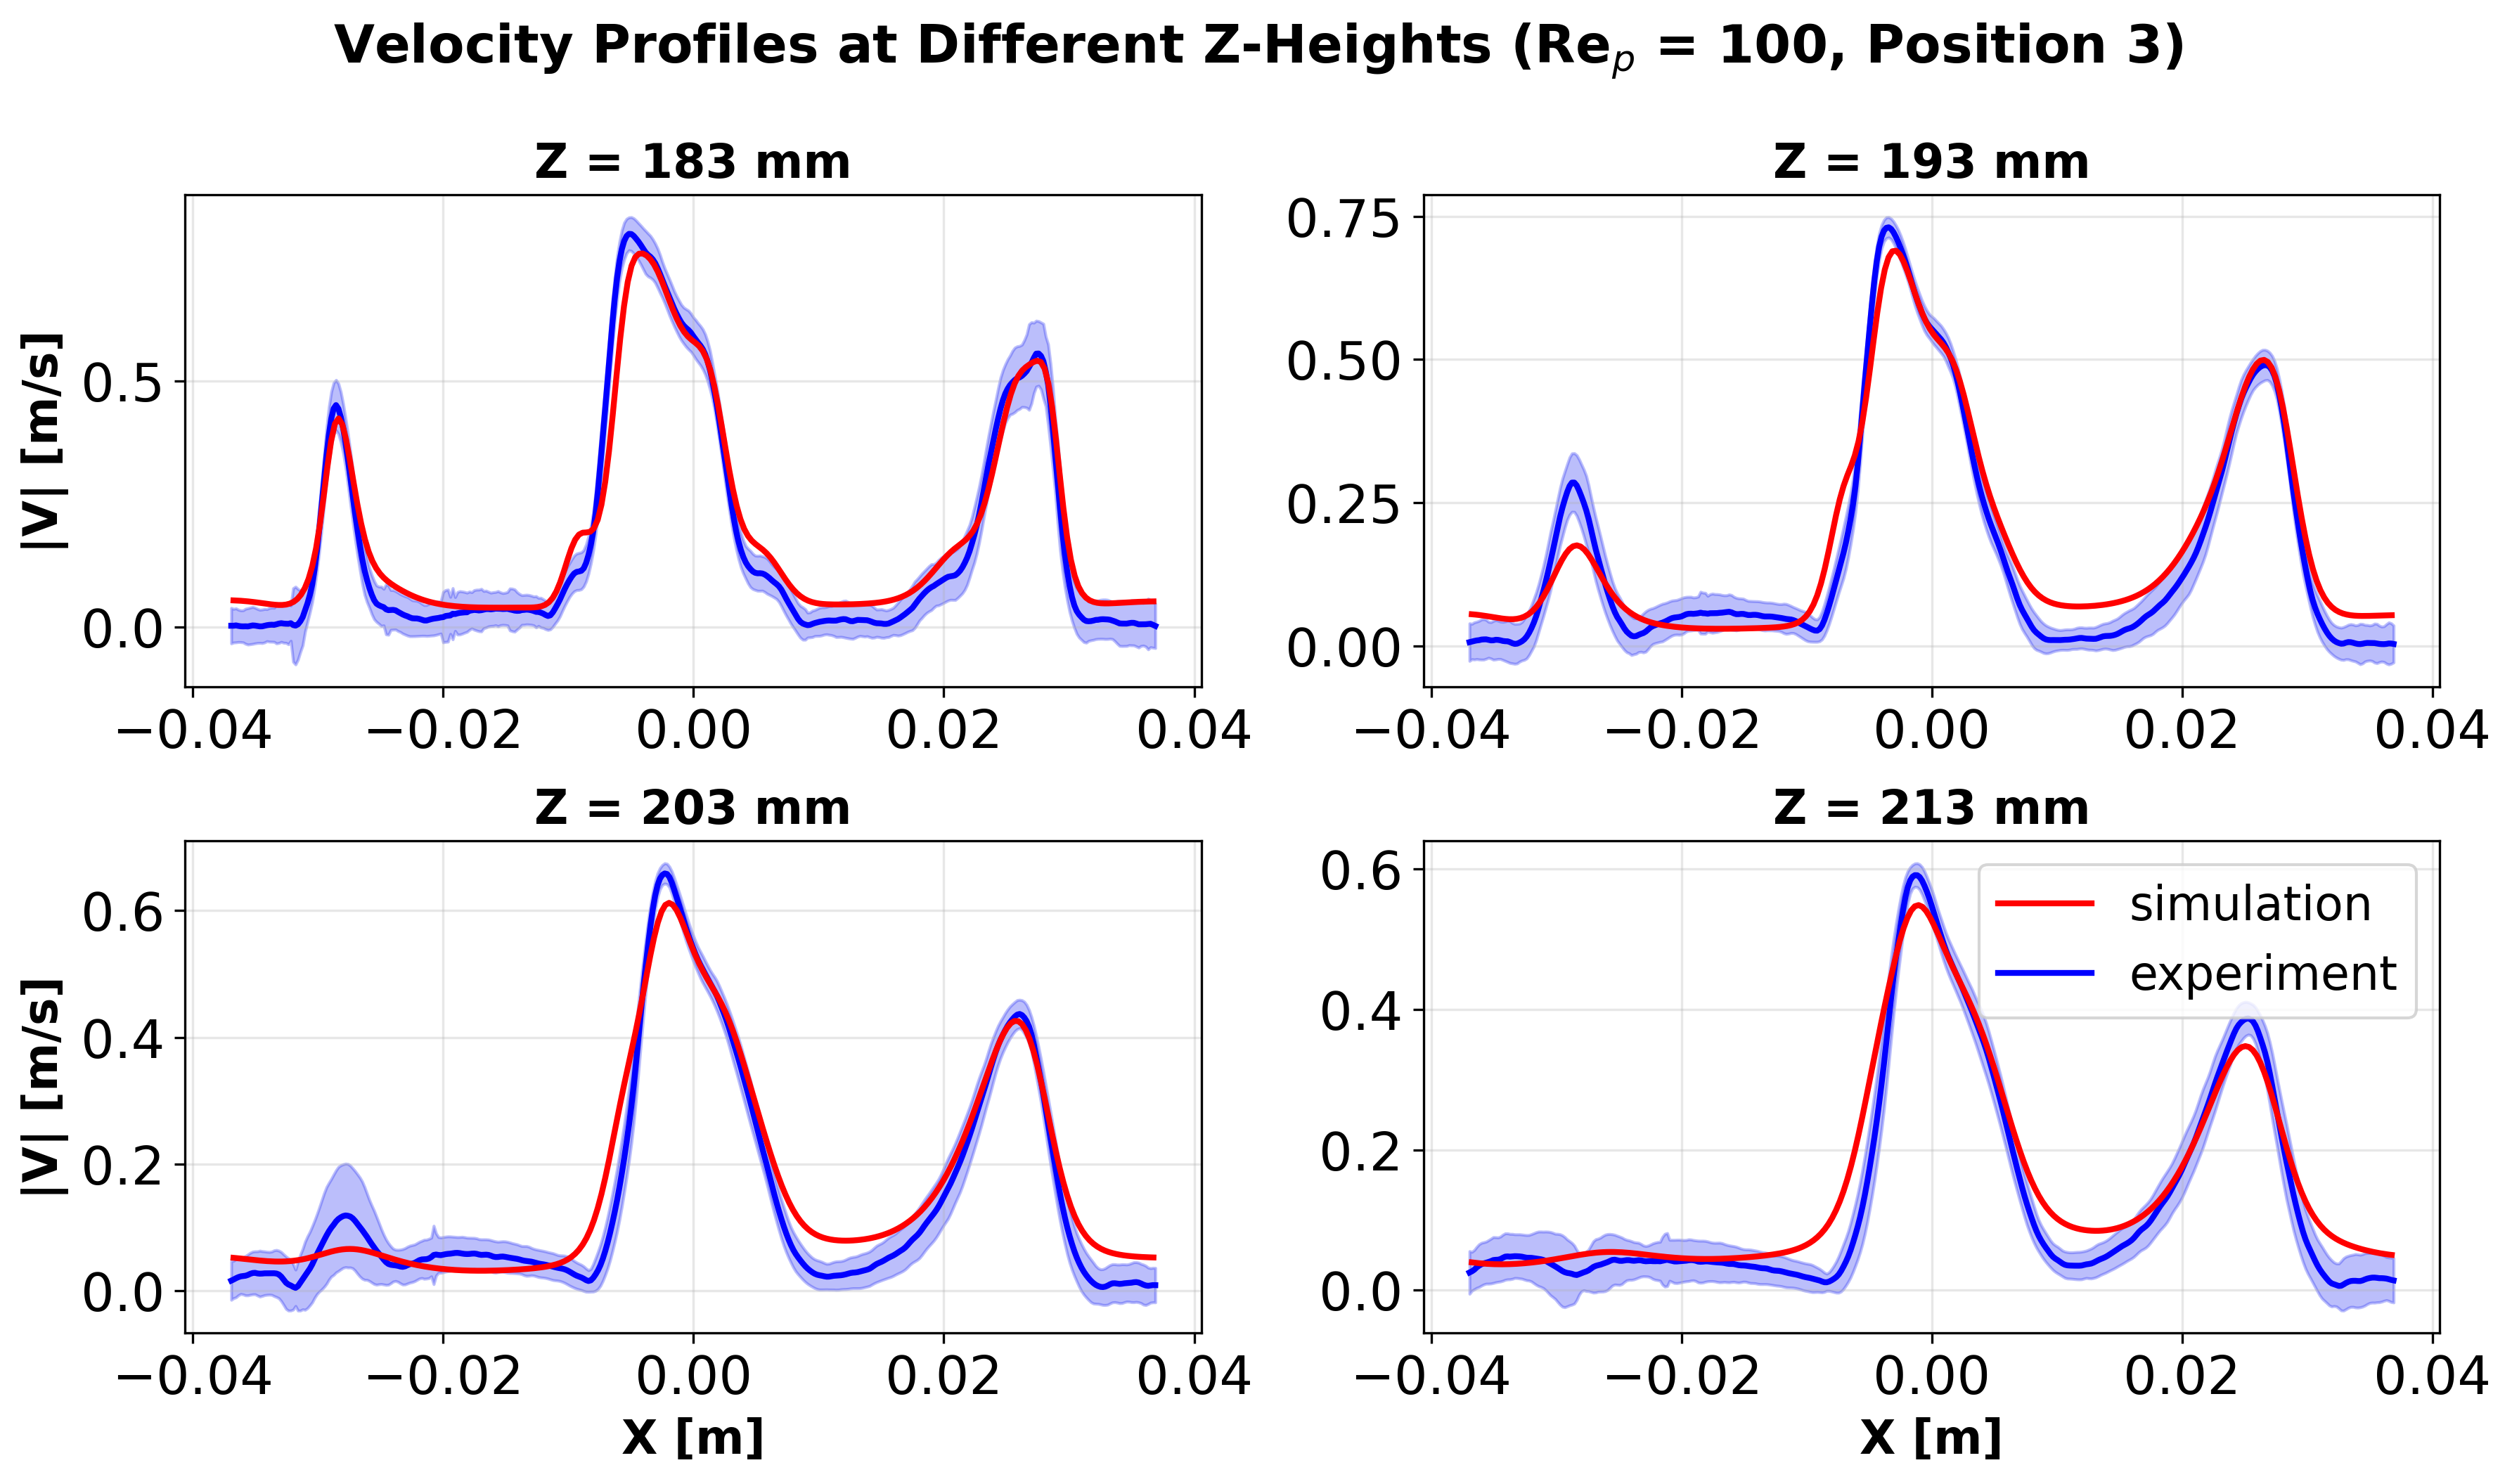
\includegraphics[width=0.95\linewidth]{30_Re_100/surface/Summary_Line_Profiles_Pos3.png}
\caption{Quantitative surface validation for the $30^\circ$ packing at $Re_P=100$,
Pos\,3: velocity-magnitude profiles across the plane at four streamwise heights,
simulation (red) versus PIV (blue) with the shaded experimental uncertainty band. The
simulated profiles lie within the measured band except in the steep shear layers
flanking the central jet.}
\label{fig:validation_profiles}
\end{figure}

\subsection{Layer-Resolved Development}
\label{sec:validation:layers}

% TODO (user supplying layer images): in-slit layer fields/profiles L13-L17,
% sim vs PIV; per-layer error; development of the locked flow layer by layer.
\todo[inline]{Layer-resolved validation: write once layer images are added (in-slit
fields/profiles L13-L17, sim vs PIV, per-layer error).}

%% ============================================================
\section{Flow Locking Framework}
\label{sec:locking}

The central, novel contribution of this paper. Prior work~\citep{velten2026} noted
qualitatively that the flow ``repeats across layers and is antisymmetric about the
central axis.'' Here that observation is turned into a measured quantity: the mean
flow repeats with the same twist as the geometry, and we score how strongly with a
single order parameter that approaches unity for the periodic packings, collapses for
the irregular packing, and weakens as the Reynolds number rises.

\subsection{Physical Interpretation: Twist-and-Repeat Flow Locking}
\label{sec:locking:concept}

% The packing has a twist-and-repeat rule: rotate by theta and shift up by one layer
% -> same structure (like a screw thread / spiral staircase).
% Flow locking means the flow obeys the same rule as the geometry.
% The irregular packing has no twist-and-repeat rule -> cannot lock -> clean control.
% Hypotheses: H1 regular packings lock with period N; H2 irregular does not lock;
% H3 locking weakens as Re_p rises toward unsteady flow.
\todo[inline]{Write §4.1 physical concept in plain language}

\subsection{Locking Order Parameter \texorpdfstring{$L(n)$}{L(n)}}
\label{sec:locking:Ln}

The locking order parameter $L(n)$ is the cosine similarity between the de-rotated
velocity fields of layer $n$ and layer $n+N$:
\begin{equation}
    L(n) = \frac{\langle \tilde{\bm{u}}_n \cdot \tilde{\bm{u}}_{n+N} \rangle}
                {\|\tilde{\bm{u}}_n\|\;\|\tilde{\bm{u}}_{n+N}\|},
    \label{eq:Ln}
\end{equation}
where $\tilde{\bm{u}}_n$ is the time-mean in-plane velocity field of layer $n$,
de-rotated by $-n\theta$ to a common reference frame, and $N = 180^\circ/\theta$ is
the layer period ($N=6$ for $\theta=30^\circ$; $N=9$ for $\theta=40^\circ$).
$L = 1$ means the de-rotated layers are identical (perfectly locked); $L \to 0$ means
no repeat. For the irregular packing (no period $N$) adjacent layers ($n \to n+1$)
are compared instead.
% Also: development length how many layers from inlet before L(n) plateaus.
\todo[inline]{Write §4.2 construction, pair-mask note, development length}

\subsection{Antisymmetry Index \texorpdfstring{$A(n)$}{A(n)}}
\label{sec:locking:An}

% A(n): cosine similarity of de-rotated field with its point-reflection about axis.
% A -> 1 (or -1 depending on sign convention) for antisymmetric locked state.
% Result: A moderate (~0.42-0.46) lead with L, treat A cautiously.
% Possibly need to revisit axis definition.
\todo[inline]{Write §4.3 antisymmetry index; revisit A definition if needed}

\subsection{Locking Across Topologies}
\label{sec:locking:topologies}

% 30 deg: L ~ 1.000 (off-diagonal matrix), de-rotated layers collapse headline.
% 40 deg: L ~ 0.99, still strong locking.
% Irregular: L = 0.10-0.68, erratic confirms geometric periodicity is required.
% Figure: Fig. 6 (visual de-rotated layer fields collapsing for 30/40, not irregular).
% Figure: Fig. 7a (L heatmap + L vs mean for all three topologies).
Figure~\ref{fig:Ln} shows the layer-to-layer locking matrix and $L(n)$ versus layer
for the three topologies.
For the 30\textdegree{} packing all off-diagonal entries are $L \approx 1.000$,
confirming near-perfect locking across the developed window (L13-L17).
The 40\textdegree{} packing locks at $L \approx 0.99$, still strongly locked but
slightly reduced owing to the larger per-layer twist angle.
The irregular packing yields $L = 0.10$-$0.68$ with no systematic pattern,
confirming that the geometric twist-and-repeat rule is a necessary condition for
flow locking.
\todo[inline]{Write §4.4 quantify L for each topology; add development curve}

\subsection{Locking Versus Reynolds Number}
\label{sec:locking:reynolds}

% Using 40 deg at Re_p = 100/300/500: track L and A as Re_p rises.
% Expected: time-mean pattern persists but locked fraction weakens.
% Bridge to Paper 2 transition study.
% Note: Re-dependence of locking only available at 40 deg in this paper.
\todo[inline]{Write §4.5 Re effect on L; insert Fig. 7d (Re trend panel)}

\subsection{Physical Interpretation and Hand-off to Paper~2}
\label{sec:locking:handoff}

% Locked flow = coherent jets spiralling with the rotating slits.
% Fully described by one layer period -> justifies the reduced 6-layer periodic domain.
\todo[inline]{Write §4.6 physical interpretation; forward pointer to Paper 2}

%% ============================================================
\section{Flow Organisation}
\label{sec:organisation}

% Where §4 establishes THAT the flow locks, §5 describes WHAT the locked flow
% looks like. Kept deliberately light on exotic diagnostics.

\subsection{Mean Flow Picture}
\label{sec:organisation:meanflow}

% Mean velocity-magnitude fields and streamlines at Pos 1 and Pos 3, layers L13-L17.
% Diagonal/spiral jet banding following the rotating slits; recirculation pockets.
% Figure: Fig. 8 (locked flow in detail, 30 deg).
\todo[inline]{Write §5.1 mean flow picture}

\subsection{Channelling and Transverse Spreading}
\label{sec:organisation:channelling}

% Channelling (flow uniformity) index: participation ratio <v>^2 / <v^2>.
% Transverse kinetic-energy fraction: (vx^2 + vy^2) / |v|^2.
% Report per layer and as packing-average.
\todo[inline]{Write §5.2 channelling index and transverse KE fraction}

\subsection{Recirculation and Secondary Motion}
\label{sec:organisation:recirculation}

% Recirculation zones behind/between bars from mean field.
% In-plane secondary-flow vectors driven by rotation.
% Optional: Q-criterion / swirling strength.
\todo[inline]{Write §5.3 recirculation; decide on optional vortex diagnostics}

\subsection{Topology Contrast: 30\textdegree{} vs 40\textdegree{} vs Irregular}
\label{sec:organisation:contrast}

% Compare on: jet strength and alignment length, channelling index, transverse-KE
% fraction, recirculation count.
% Expected story: 30 deg = most coherent jets; 40 deg = more cross-flow redistribution;
% irregular = erratic transport, no organised jets.
% Figure: Fig. 9 (topology contrast, same plane same scale).
% Figure: Fig. 10 (summary metrics bar/scatter).
\todo[inline]{Write §5.4 topology contrast; insert Figs. 9 and 10}

%% ============================================================
\section{Conclusions}
\label{sec:conclusions}

% 3-4 bullets tied directly to novelty claims:
% 1. First pore-scale LBM of Ref Config IIa, validated vs PIV across 3 topologies (~2.5%).
% 2. Flow locking is real, measurable, and topology-controlled (L ~ 1 for regular; collapses for irregular).
% 3. Irregular packing breaks locking confirms geometric periodicity is the necessary condition.
% 4. The 6-layer periodicity justifies the reduced periodic domain used in Paper 2.
\todo[inline]{Write Conclusions}

%% ============================================================
\begin{thebibliography}{}

\bibitem{Bao}
Bao, Y. (2019). Recent advances in the lattice Boltzmann method: A review. Journal of Engineering Thermophysics, 28(4), 711-722.

\bibitem{Rahman}
Rahman, M.~M., \& Bao, Y. (2017). Numerical simulation of flow through porous media using the lattice Boltzmann method. Journal of Petroleum Science and Engineering, 158, 411-425.

\bibitem{Kruger}
Kr\"{u}ger, T., Varnik, F., \& Raabe, D. Efficient and accurate simulations of deformable particles immersed in a fluid using a combined immersed boundary lattice Boltzmann finite element method. Computers \& Mathematics with Applications, 61, 3485-3505. (2011)

\bibitem{Young}
Young-Il Lim. Computational Fluid Dynamics (CFD) of Chemical Processes. (2006).

\bibitem{Aglave}
Aglave, R., Eppinger, T., \& Jurtz, N. Automated workflow for spatially resolved fixed bed reactors with spherical and non-spherical particles. (2014).

\bibitem{Ying}
Dong, Y., Korup, O., Gerdts, J., Rold\'{a}n Cuenya, B., \& Horn, R. Microtomography-based CFD modeling of a fixed-bed reactor with an open-cell foam monolith and experimental verification by reactor profile measurements. Chemical Engineering Journal, 353, 176-188. (2018)

\bibitem{Fattahi}
Fattahi, E., Waluga, C., Wohlmuth, B., R\"{u}de, U., Manhart, M., \& Helmig, R. Lattice Boltzmann methods in porous media simulations: From laminar to turbulent flow. Computers \& Fluids, 140. (2016).

\bibitem{Sullivan}
Sullivan, S.~P., Sani, F.~M., Johns, M.~L., \& Gladden, L.~F. Simulation of packed bed reactors using lattice Boltzmann methods. Chemical Engineering Science, 60(12), 3405-3418. (2005).

\bibitem{Sukop}
Sukop, M., \& Or, D. Lattice Boltzmann method for modeling liquid-vapor interface configurations in porous media. Water Resources Research, 40. (2004).

\bibitem{Shi}
Shi, L., Yu, Z., \& Jaworski, A.~J. Investigation into the Strouhal numbers associated with vortex shedding from parallel-plate thermoacoustic stacks in oscillatory flow conditions. European Journal of Mechanics, B/Fluids, 30(2), 206-217. (2011)

\bibitem{Yoshida}
Yoshida, H., \& Nagaoka, M. Multiple-relaxation-time lattice Boltzmann model for the convection and anisotropic diffusion equation. Journal of Computational Physics, 229, 7774-7795. (2010).

\bibitem{Dixon}
Dixon, A.~G., \& Partopour, B. Computational fluid dynamics for fixed bed reactor design. Annual Review of Chemical and Biomolecular Engineering, 11, 109-130. (2020)

\bibitem{Hosseini}
S.~A. Hosseini. Development of a lattice Boltzmann-based numerical method for the simulation of reacting flows. PhD thesis, Universit\'{e} Paris-Saclay \& Otto-von-Guericke university. (2020)

\bibitem{Xiaoyi}
He, X., \& Luo, L.-S. Theory of the lattice Boltzmann method: From the Boltzmann equation to the lattice Boltzmann equation. Physical Review E, 56, 6811-6817. (1997).

\bibitem{Shu}
Xiaoyi, G., \& Shu, C. Lattice Boltzmann Method and Its Applications in Engineering. World Scientific Publishing Company. (2012).

\bibitem{hosseini2020compressibility}
Hosseini, S.~A., Darabiha, N., \& Th\'{e}venin, D. Compressibility in lattice {Boltzmann} on standard stencils: effects of deviation from reference temperature. Philosophical Transactions of the Royal Society A, 378, 20190399. (2020)

\bibitem{feng2015three}
Feng, Y., Sagaut, P., \& Tao, W. A three-dimensional lattice model for thermal compressible flow on standard lattices. Journal of Computational Physics, 303, 514-529. (2015).

\bibitem{hosseini2022lattice}
Hosseini, S.~A., Huang, F., \& Thevenin, D. Lattice Boltzmann model for simulation of flow in intracranial aneurysms considering non-Newtonian effects. Physics of Fluids, 34(7), 073105. (2022).

\bibitem{huang2022simulation}
Huang, F., Noel, R., Berg, P., \& Hosseini, S.~A. Simulation of the FDA nozzle benchmark: A lattice Boltzmann study. Computer Methods and Programs in Biomedicine, 221, 106863. (2022).

\bibitem{neeraj2023}
Neeraj, T., Velten, C., Janiga, G., et al. Modeling gas flows in packed beds with the lattice {Boltzmann} method: validation against experiments. Flow, Turbulence and Combustion, 111, 463-491. (2023). \url{https://doi.org/10.1007/s10494-023-00444-z}

\bibitem{hosseini2021central}
Hosseini, S.~A., Berg, P., Huang, F., Roloff, C., Janiga, G., \& Thevenin, D. Central moments multiple relaxation time LBM for hemodynamic simulations in intracranial aneurysms: An in-vitro validation study using PIV and PC-MRI. Computers in Biology and Medicine, 131, 104251. (2021).

\bibitem{Bhadauria}
Bhadauria, B.~S. Lattice Boltzmann Method Fundamentals and Engineering Applications with Computer Codes. Springer Science \& Business Media. (2009).

\bibitem{Boutt}
Boutt, D.~F., et al. Direct simulation of fluid-solid mechanics in porous media using the discrete element and lattice-Boltzmann methods. Journal of Geophysical Research: Solid Earth, 112, B10. (2007).

\bibitem{Kawamura}
Kawamura, H., Abe, H., \& Shingai, K. DNS of turbulence and heat transport in a channel flow with different Reynolds and Prandtl numbers and boundary conditions. Proceedings of the 3rd International Symposium on Turbulence, Heat and Mass Transfer. (2000).

\bibitem{kruger2017lattice}
Krueger, T., Kusumaatmaja, H., Kuzmin, A., Shardt, O., Silva, G., \& Viggen, E.~M. The Lattice Boltzmann Method: Principles and Practice. Springer. (2016).

\bibitem{bouzidi2001momentum}
Bouzidi, M., Firdaouss, M., \& Lallemand, P. Momentum transfer of a {Boltzmann}-lattice fluid with boundaries. Physics of Fluids, 13(11), 3452-3459. (2001).

\bibitem{zhao2002non}
Zhao-Li, G., Chu-Guang, Z., \& Bao-Chang, S. Non-equilibrium extrapolation method for velocity and pressure boundary conditions in the lattice {Boltzmann} method. Chinese Physics, 11(4), 366. (2002).

\bibitem[Velten et al.(2026)]{velten2026}
Velten, C., H\"{u}lz, K., \& Z\"{a}hringer, K. Allowing optical measurements in a {3D} packed bed with gas flow: {A} novel reactor concept. \textit{Particuology}, 108, 293-306. (2026). \url{https://doi.org/10.1016/j.partic.2025.11.018} (Open Access, CC~BY~4.0)

\bibitem{velten2022a}
Velten, C., Ebert, M., Lessig, C., \& Z\"{a}hringer, K. Ray tracing based reconstruction of PIV measurements in the outlet zone of gaseous flow in packed beds. 20th International Symposium on the Application of Laser and Imaging Techniques to Fluid Mechanics, Lisbon, Portugal. (2022a).

\bibitem{velten2022b}
Velten, C., Ebert, M., Lessig, C., \& Z\"{a}hringer, K. Ray tracing particle image velocimetry challenges in the application to a packed bed. (2022b).

\end{thebibliography}

\end{document}
